\section{Parte A - Planificación de Operaciones}
\label{sec:parteA}

\begin{center}
\fbox{\begin{minipage}{0.9\textwidth}
    \textbf{Descripción de la Parte A:} \\
    En esta parte de la tarea se aborda el modelamiento y resolución del problema de optimización para la Fundación Circular, una iniciativa de reacondicionamiento de ropa donada para comunidades vulnerables. Se desarrolla un modelo de optimización lineal para minimizar los costos totales de operación y se analiza la solución óptima obtenida.
\end{minipage}}
\end{center}

\vspace{1cm}

\subsection*{Introducción a la Parte A}

La Fundación Circular ha lanzado una iniciativa para reacondicionar ropa donada y entregarla a comunidades vulnerables. El problema se centra en la gestión eficiente de una planta que recibe donaciones de ropa, las procesa y satisface demandas de prendas. En esta parte, se desarrolla un modelo de optimización lineal para minimizar los costos totales de operación y se analiza la solución obtenida.

\begin{itemize}
    \item \textbf{Pregunta 1:} Modelamiento del problema mediante optimización lineal
    \item \textbf{Pregunta 2:} Resolución del modelo y análisis de resultados
    \item \textbf{Pregunta 3:} Evaluación del modelo bajo falla en maquinaria
    \item \textbf{Pregunta 4:} Análisis de estrategia de adquisición de ropa usada
    \item \textbf{Pregunta 5:} Evaluación de dotación de personal variable
    \item \textbf{Pregunta 6:} Análisis de sensibilidad del modelo
\end{itemize}

\question{1}
\label{q:pregunta1}

% Descripción de la pregunta
Modele el problema mediante optimización lineal, explicando el significado de parámetros, variables, función objetivo y restricciones utilizadas.

\answer

\subsection*{Contexto del problema}

La Fundación Circular ha lanzado una iniciativa para reacondicionar ropa donada y entregarla a comunidades vulnerables. El problema se centra en la gestión eficiente de una planta que:

\begin{itemize}
    \item Recibe donaciones de ropa en buen y mal estado
    \item Transforma ropa en mal estado en género textil
    \item Produce nuevas prendas a partir del género textil
    \item Satisface demandas de prendas en cada periodo
\end{itemize}

El objetivo es minimizar los costos totales de operación sobre un horizonte de planificación definido, considerando costos de personal, procesamiento, almacenamiento y penalizaciones por demandas no satisfechas.

\subsection*{Conjuntos e índices}

\begin{itemize}
    \item $T$: Conjunto de periodos del horizonte de planificación, indexado por $t \in \{1,2,...,T\}$
\end{itemize}

\subsection*{Parámetros}

\subsubsection*{Parámetros de entrada de materiales}

\begin{itemize}
    \item $kb_t$: Kilogramos de ropa en buen estado que llegan en el periodo $t$
    \item $km_t$: Kilogramos de ropa en mal estado que llegan en el periodo $t$
    \item $rb$: Inventario inicial de ropa en buen estado (kg)
    \item $rm$: Inventario inicial de ropa en mal estado (kg)
    \item $p$: Peso promedio de cada unidad de ropa (kg/prenda)
\end{itemize}

\subsubsection*{Parámetros de demanda}

\begin{itemize}
    \item $d_t$: Demanda de prendas para el periodo $t$
    \item $cp$: Costo de penalización por demanda no satisfecha (\$/prenda)
\end{itemize}

\subsubsection*{Parámetros de costos}

\begin{itemize}
    \item $ct$: Costo por trabajador contratado por boleta (\$/persona/periodo)
    \item $g$: Costo unitario de transformación a género (\$/kg)
    \item $n$: Costo unitario de producción de prendas desde género (\$/kg)
    \item $a$: Costo de almacenamiento (\$/kg/periodo)
    \item $cc$: Costo por hora normal trabajada (\$/hora)
\end{itemize}

\subsubsection*{Parámetros de capacidad}

\begin{itemize}
    \item $s$: Capacidad máxima de almacenamiento (kg)
    \item $w_0$: Dotación inicial de trabajadores
    \item $h$: Horas de trabajo por trabajador por periodo
    \item $\tau_g$: Horas-hombre para transformar 1 kg de ropa en mal estado a género
    \item $\tau_n$: Horas-hombre para confeccionar 1 kg de ropa reutilizada desde género
\end{itemize}

\subsection*{Variables de decisión}

\subsubsection*{Variables de procesamiento y producción}

\begin{itemize}
    \item $X_{t}$: Kilogramos de ropa en buen estado utilizados para satisfacer demanda en periodo $t$
    \begin{itemize}
        \item Justificación: Representa el flujo principal de ropa en buen estado que se destina directamente para satisfacer la demanda.
        \item Unidades: Kilogramos (kg)
        \item Dominio: $X_t \geq 0$ (variable continua no negativa)
    \end{itemize}

    \item $Y_{t}$: Kilogramos de ropa en mal estado transformados a género en periodo $t$
    \begin{itemize}
        \item Justificación: Representa la cantidad de ropa en mal estado que se procesa para obtener género textil.
        \item Unidades: Kilogramos (kg)
        \item Dominio: $Y_t \geq 0$ (variable continua no negativa)
    \end{itemize}

    \item $Z_{t}$: Kilogramos de género utilizados para fabricar prendas en periodo $t$
    \begin{itemize}
        \item Justificación: Representa la cantidad de género que se utiliza para producir prendas reutilizadas.
        \item Unidades: Kilogramos (kg)
        \item Dominio: $Z_t \geq 0$ (variable continua no negativa)
    \end{itemize}
\end{itemize}

\subsubsection*{Variables de inventario}

\begin{itemize}
    \item $IB_{t}$: Inventario de ropa en buen estado al final del periodo $t$
    \begin{itemize}
        \item Justificación: Control del stock de ropa en buen estado disponible entre periodos.
        \item Unidades: Kilogramos (kg)
        \item Dominio: $IB_t \geq 0$ (variable continua no negativa)
    \end{itemize}

    \item $IM_{t}$: Inventario de ropa en mal estado al final del periodo $t$
    \begin{itemize}
        \item Justificación: Control del stock de ropa en mal estado disponible entre periodos.
        \item Unidades: Kilogramos (kg)
        \item Dominio: $IM_t \geq 0$ (variable continua no negativa)
    \end{itemize}

    \item $IG_{t}$: Inventario de género al final del periodo $t$
    \begin{itemize}
        \item Justificación: Control del stock de género textil disponible entre periodos.
        \item Unidades: Kilogramos (kg)
        \item Dominio: $IG_t \geq 0$ (variable continua no negativa)
    \end{itemize}
\end{itemize}

\subsubsection*{Variables de recursos humanos}

\begin{itemize}
    \item $W_{t}$: Número de trabajadores por boleta contratados en periodo $t$
    \begin{itemize}
        \item Justificación: Representa la fuerza laboral adicional contratada para satisfacer la demanda de mano de obra.
        \item Unidades: Personas (trabajadores)
        \item Dominio: $W_t \geq 0$, entero (variable entera no negativa)
    \end{itemize}
\end{itemize}

\subsubsection*{Variables de satisfacción de demanda}

\begin{itemize}
    \item $NS_{t}$: Demanda no satisfecha en periodo $t$
    \begin{itemize}
        \item Justificación: Mide la cantidad de demanda que no puede ser cubierta durante el periodo.
        \item Unidades: Prendas
        \item Dominio: $NS_t \geq 0$ (variable continua no negativa)
    \end{itemize}
\end{itemize}

\subsection*{Función objetivo}

Minimizar el costo total de la operación:

\begin{equation}
\min Z = \sum_{t=1}^{T} \left[ W_t \cdot ct + cc \cdot h \cdot w_0 + g \cdot Y_t + n \cdot Z_t + a \cdot (IB_t + IM_t + IG_t) + cp \cdot NS_t \right]
\end{equation}

Esta función objetivo integra todos los componentes de costo que la Fundación Circular busca minimizar:

\subsubsection*{Desglose de la función objetivo}

\begin{enumerate}
    \item \textbf{Costos de personal}:
    \begin{itemize}
        \item $W_t \cdot ct$: Costo de los trabajadores contratados por boleta en cada periodo $t$
        \item $cc \cdot h \cdot w_0$: Costo fijo de la dotación inicial de trabajadores contratados
        \item Justificación: Representa el gasto en recursos humanos, diferenciando entre personal fijo y temporal
    \end{itemize}

    \item \textbf{Costos de procesamiento}:
    \begin{itemize}
        \item $g \cdot Y_t$: Costo de transformar ropa en mal estado a género textil
        \item $n \cdot Z_t$: Costo de producir prendas a partir de género textil
        \item Justificación: Captura los costos variables asociados a los procesos productivos principales
    \end{itemize}

    \item \textbf{Costos de almacenamiento}:
    \begin{itemize}
        \item $a \cdot (IB_t + IM_t + IG_t)$: Costo de mantener inventarios de los tres tipos de materiales
        \item Justificación: Refleja los costos de mantener stock entre periodos, aplicando el mismo costo unitario a todos los tipos de materiales conforme al enunciado
    \end{itemize}

    \item \textbf{Costos de penalización}:
    \begin{itemize}
        \item $cp \cdot NS_t$: Penalización por demanda no satisfecha
        \item Justificación: Incorpora el costo social/económico de no entregar las prendas comprometidas
    \end{itemize}
\end{enumerate}

\subsection*{Restricciones}

\subsubsection*{Restricciones de balance de inventario}

Estas restricciones garantizan la conservación del flujo de materiales entre periodos consecutivos.

\paragraph{Balance de inventario de ropa en buen estado}

\begin{equation}
IB_t = IB_{t-1} + kb_t - X_t \quad \forall t \in T
\end{equation}

Donde:
\begin{itemize}
    \item $IB_0 = rb$ (inventario inicial de ropa en buen estado)
\end{itemize}

\textbf{Interpretación}: El inventario de ropa en buen estado al final del periodo $t$ es igual al inventario del periodo anterior, más las llegadas de ropa en buen estado en el periodo actual, menos la cantidad utilizada para satisfacer demanda.

\paragraph{Balance de inventario de ropa en mal estado}

\begin{equation}
IM_t = IM_{t-1} + km_t - Y_t \quad \forall t \in T
\end{equation}

Donde:
\begin{itemize}
    \item $IM_0 = rm$ (inventario inicial de ropa en mal estado)
\end{itemize}

\textbf{Interpretación}: El inventario de ropa en mal estado al final del periodo $t$ es igual al inventario del periodo anterior, más las llegadas de ropa en mal estado en el periodo actual, menos la cantidad transformada a género.

\paragraph{Balance de inventario de género}

\begin{equation}
IG_t = IG_{t-1} + Y_t - Z_t \quad \forall t \in T
\end{equation}

Donde:
\begin{itemize}
    \item $IG_0 = 0$ (se asume que no hay inventario inicial de género)
\end{itemize}

\textbf{Interpretación}: El inventario de género textil al final del periodo $t$ es igual al inventario del periodo anterior, más la cantidad producida por transformación de ropa en mal estado, menos la cantidad utilizada para fabricar prendas.

\subsubsection*{Restricción de capacidad de almacenamiento}

\begin{equation}
IB_t + IM_t + IG_t \leq s \quad \forall t \in T
\end{equation}

\textbf{Interpretación}: La suma de todos los inventarios al final de cada periodo no puede exceder la capacidad máxima de almacenamiento disponible ($s$ kg). Esta restricción asegura que la fundación no sobrepase su infraestructura de almacenamiento.

\subsubsection*{Restricción de disponibilidad de horas-hombre}

\begin{equation}
\tau_g \cdot Y_t + \tau_n \cdot Z_t \leq h \cdot (w_0 + W_t) \quad \forall t \in T
\end{equation}

\textbf{Interpretación}: El tiempo total requerido para las operaciones de transformación de ropa a género ($\tau_g \cdot Y_t$) y fabricación de prendas desde género ($\tau_n \cdot Z_t$) no puede exceder la disponibilidad total de horas-hombre, determinada por el número total de trabajadores (contratados $w_0$ y por boleta $W_t$) multiplicado por las horas disponibles por trabajador ($h$).

\subsubsection*{Restricción de satisfacción de la demanda}

\begin{equation}
\frac{X_t}{p} + \frac{Z_t}{p} + NS_t \geq d_t \quad \forall t \in T
\end{equation}

\textbf{Interpretación}: La demanda de prendas en cada periodo debe ser satisfecha mediante:
\begin{itemize}
    \item Prendas de ropa en buen estado ($\frac{X_t}{p}$ prendas, considerando que cada prenda pesa $p$ kg)
    \item Prendas fabricadas a partir de género ($\frac{Z_t}{p}$ prendas)
    \item Demanda no satisfecha ($NS_t$ prendas), que conlleva una penalización
\end{itemize}

\subsubsection*{Restricciones de dominio de variables}

\begin{align}
X_t, Y_t, Z_t, IB_t, IM_t, IG_t &\geq 0 \quad \forall t \in T\\
W_t &\geq 0, \text{ entero} \quad \forall t \in T\\
NS_t &\geq 0 \quad \forall t \in T
\end{align}

\subsection*{Justificación del modelo}

Este modelo de optimización lineal captura todos los aspectos relevantes del problema de la Fundación Circular de manera comprehensiva:

\begin{enumerate}
    \item \textbf{Alineación con los objetivos de la fundación}
    
    El modelo está diseñado para minimizar los costos totales de operación mientras se gestionan eficientemente los recursos disponibles y se satisface la demanda de prendas para comunidades vulnerables. Esto se alinea perfectamente con el objetivo social de la fundación y su necesidad de operar de manera sostenible económicamente.

    \item \textbf{Representación integral del sistema productivo}
    
    El modelo representa de manera completa el flujo de materiales y procesos de la Fundación Circular:
    \begin{itemize}
        \item \textbf{Sistema de tres flujos de materiales}: Ropa en buen estado, ropa en mal estado y género textil
        \item \textbf{Procesos de transformación}: Conversión de ropa en mal estado a género y producción de prendas a partir de género
        \item \textbf{Gestión de inventarios}: Control de stocks entre periodos con sus costos asociados
        \item \textbf{Administración de recursos humanos}: Balance entre trabajadores fijos y contratados por periodo
    \end{itemize}
\end{enumerate}

\subsection*{Supuestos y limitaciones del modelo}

\subsubsection*{Supuestos}
\begin{itemize}
    \item \textbf{Relaciones de peso constantes}: La transformación de ropa en mal estado a género y la fabricación de prendas desde género tienen una relación de 1:1 en términos de peso.
    \item \textbf{Homogeneidad de prendas}: Todas las prendas tienen el mismo peso promedio $p$.
    \item \textbf{Disponibilidad ilimitada de trabajadores por boleta}: No hay restricciones en la cantidad máxima de trabajadores por boleta que se pueden contratar.
    \item \textbf{Linealidad de costos y tiempos}: Todos los costos y tiempos de procesamiento son lineales respecto a las cantidades procesadas.
\end{itemize}

\subsubsection*{Limitaciones}
\begin{itemize}
    \item \textbf{Determinístico}: No considera incertidumbre en parámetros como demanda o llegadas de donaciones.
    \item \textbf{Homogeneidad}: No distingue entre diferentes tipos o calidades de prendas.
    \item \textbf{Linealidad}: Asume relaciones lineales que podrían no reflejar completamente la realidad.
    \item \textbf{Horizonte fijo}: Opera con un horizonte de planificación predefinido, sin considerar efectos posteriores.
\end{itemize}
% Pregunta 2 - Resolución
\question{2}
\label{q:pregunta2}

% Descripción de la pregunta
Resuelva el modelo formulado en la pregunta 1, utilizando los valores indicados en el archivo de parámetros. Presente de manera clara los resultados obtenidos, destacando el valor de la función objetivo y la interpretación de las variables de decisión utilizadas. Realice un análisis de los resultados.

\answer

\subsection*{Resumen de resultados}

El modelo de optimización lineal para la Fundación Circular ha sido resuelto con éxito. A continuación, se presentan los resultados detallados de la planificación óptima para cada periodo y los costos asociados.

\subsubsection*{Planificación de producción y procesamiento}

\begin{table}[H]
\centering
\caption{Planificación de producción y satisfacción de demanda por periodo}
\label{tab:produccion}
\csvreader[
    tabular=ccccccc,
    table head=\toprule \textbf{Periodo} & \textbf{\begin{tabular}[c]{@{}c@{}}Ropa buen\\estado (kg)\end{tabular}} & \textbf{\begin{tabular}[c]{@{}c@{}}Ropa mal\\estado (kg)\end{tabular}} & \textbf{\begin{tabular}[c]{@{}c@{}}Género\\utilizado (kg)\end{tabular}} & \textbf{\begin{tabular}[c]{@{}c@{}}Prendas\\producidas\end{tabular}} & \textbf{\begin{tabular}[c]{@{}c@{}}Demanda\\satisfecha\end{tabular}} & \textbf{\begin{tabular}[c]{@{}c@{}}Demanda\\insatisfecha\end{tabular}} \\\midrule,
    command=\$\num{#2}\$ & \$\num{#3}\$ & \$\num{#4}\$ & \$\num{#5}\$ & \$\num{#6}\$ & \$\num{#7}\$,
    late after line=\\,
    table foot=\bottomrule,
    respect dollar=false,
    respect percent=false
]{resources/pregunta2/resultados_tabla1_p2.csv}{}{}
\end{table}

\subsubsection*{Inventarios al final de cada periodo}

\begin{table}[H]
\centering
\caption{Evolución de inventarios por periodo}
\label{tab:inventarios}
\csvreader[
    tabular=cccccc,
    table head=\toprule \textbf{Periodo} & \textbf{\begin{tabular}[c]{@{}c@{}}Inv. ropa\\buen estado (kg)\end{tabular}} & \textbf{\begin{tabular}[c]{@{}c@{}}Inv. ropa\\mal estado (kg)\end{tabular}} & \textbf{\begin{tabular}[c]{@{}c@{}}Inv. género\\(kg)\end{tabular}} & \textbf{\begin{tabular}[c]{@{}c@{}}Almacenamiento\\total (kg)\end{tabular}} & \textbf{\begin{tabular}[c]{@{}c@{}}\% Capacidad\\utilizada\end{tabular}} \\\midrule,
    command=\$\num{#1}\$ & \$\num{#2}\$ & \$\num{#3}\$ & \$\num{#4}\$ & \$\num{#5}\$ & \$\num{#6}\$,
    late after line=\\,
    table foot=\bottomrule,
    respect dollar=false,
    respect percent=false
]{resources/pregunta2/resultados_tabla2_p2.csv}{}{}
\end{table}

\subsubsection*{Recursos humanos y utilización}

\begin{table}[H]
\centering
\caption{Planificación de recursos humanos por periodo}
\label{tab:rrhh}
\begin{tabular}{ccccccc}
\toprule
\textbf{Periodo} & \textbf{\begin{tabular}[c]{@{}c@{}}Trabajadores\\contratados\end{tabular}} & \textbf{\begin{tabular}[c]{@{}c@{}}Trabajadores\\por boleta\end{tabular}} & \textbf{\begin{tabular}[c]{@{}c@{}}Total\\trabajadores\end{tabular}} & \textbf{\begin{tabular}[c]{@{}c@{}}Horas\\disponibles\end{tabular}} & \textbf{\begin{tabular}[c]{@{}c@{}}Horas\\utilizadas\end{tabular}} & \textbf{\begin{tabular}[c]{@{}c@{}}\%\\Utilización\end{tabular}} \\
\midrule
1 & $2$ & $2$ & $4$ & $32.00$ & $32.00$ & $100.00$ \\
2 & $2$ & $1$ & $3$ & $24.00$ & $24.00$ & $100.00$ \\
3 & $2$ & $2$ & $4$ & $32.00$ & $32.00$ & $100.00$ \\
4 & $2$ & $0$ & $2$ & $16.00$ & $16.00$ & $100.00$ \\
5 & $2$ & $0$ & $2$ & $16.00$ & $16.00$ & $100.00$ \\
\textbf{Total} & $\mathbf{10}$ & $\mathbf{5}$ & $\mathbf{15}$ & $\mathbf{120.00}$ & $\mathbf{120.00}$ & $\mathbf{100.00}$ \\
\bottomrule
\end{tabular}
\end{table}

\subsubsection*{Desglose de costos}

\begin{table}[H]
\centering
\caption{Componentes del costo total}
\label{tab:costos}
\begin{tabular}{cccc}
\toprule
\textbf{Componente} & \textbf{Fórmula} & \textbf{Valor (\$)} & \textbf{Porcentaje} \\
\midrule
Personal contratado & $cc*h*w0*T = 11500.0*8.0*2*5$ & $920,000.00$ & $10.03\%$ \\
Personal por boleta & $ct*\sum W_t = 215000.0*5$ & $1,075,000.00$ & $11.72\%$ \\
Transformación a género & $g*\sum Y_t = 395.0*333.33$ & $131,666.67$ & $1.44\%$ \\
Producción de prendas & $n*\sum Z_t = 265.0*333.33$ & $88,333.33$ & $0.96\%$ \\
Almacenamiento & $a*\sum(IB_t+IM_t+IG_t) = 405.0*33.89$ & $13,725.00$ & $0.15\%$ \\
Penalización & $cp*\sum NS_t = 7000.0*991.67$ & $6,941,666.69$ & $75.70\%$ \\
\midrule
\textbf{Costo total} & \textbf{Suma de todos los componentes} & $\mathbf{9,170,391.69}$ & $\mathbf{100.00\%}$ \\
\bottomrule
\end{tabular}
\end{table}

% Incluir imágenes/gráficos relevantes
\begin{figure}[H]
    \centering
    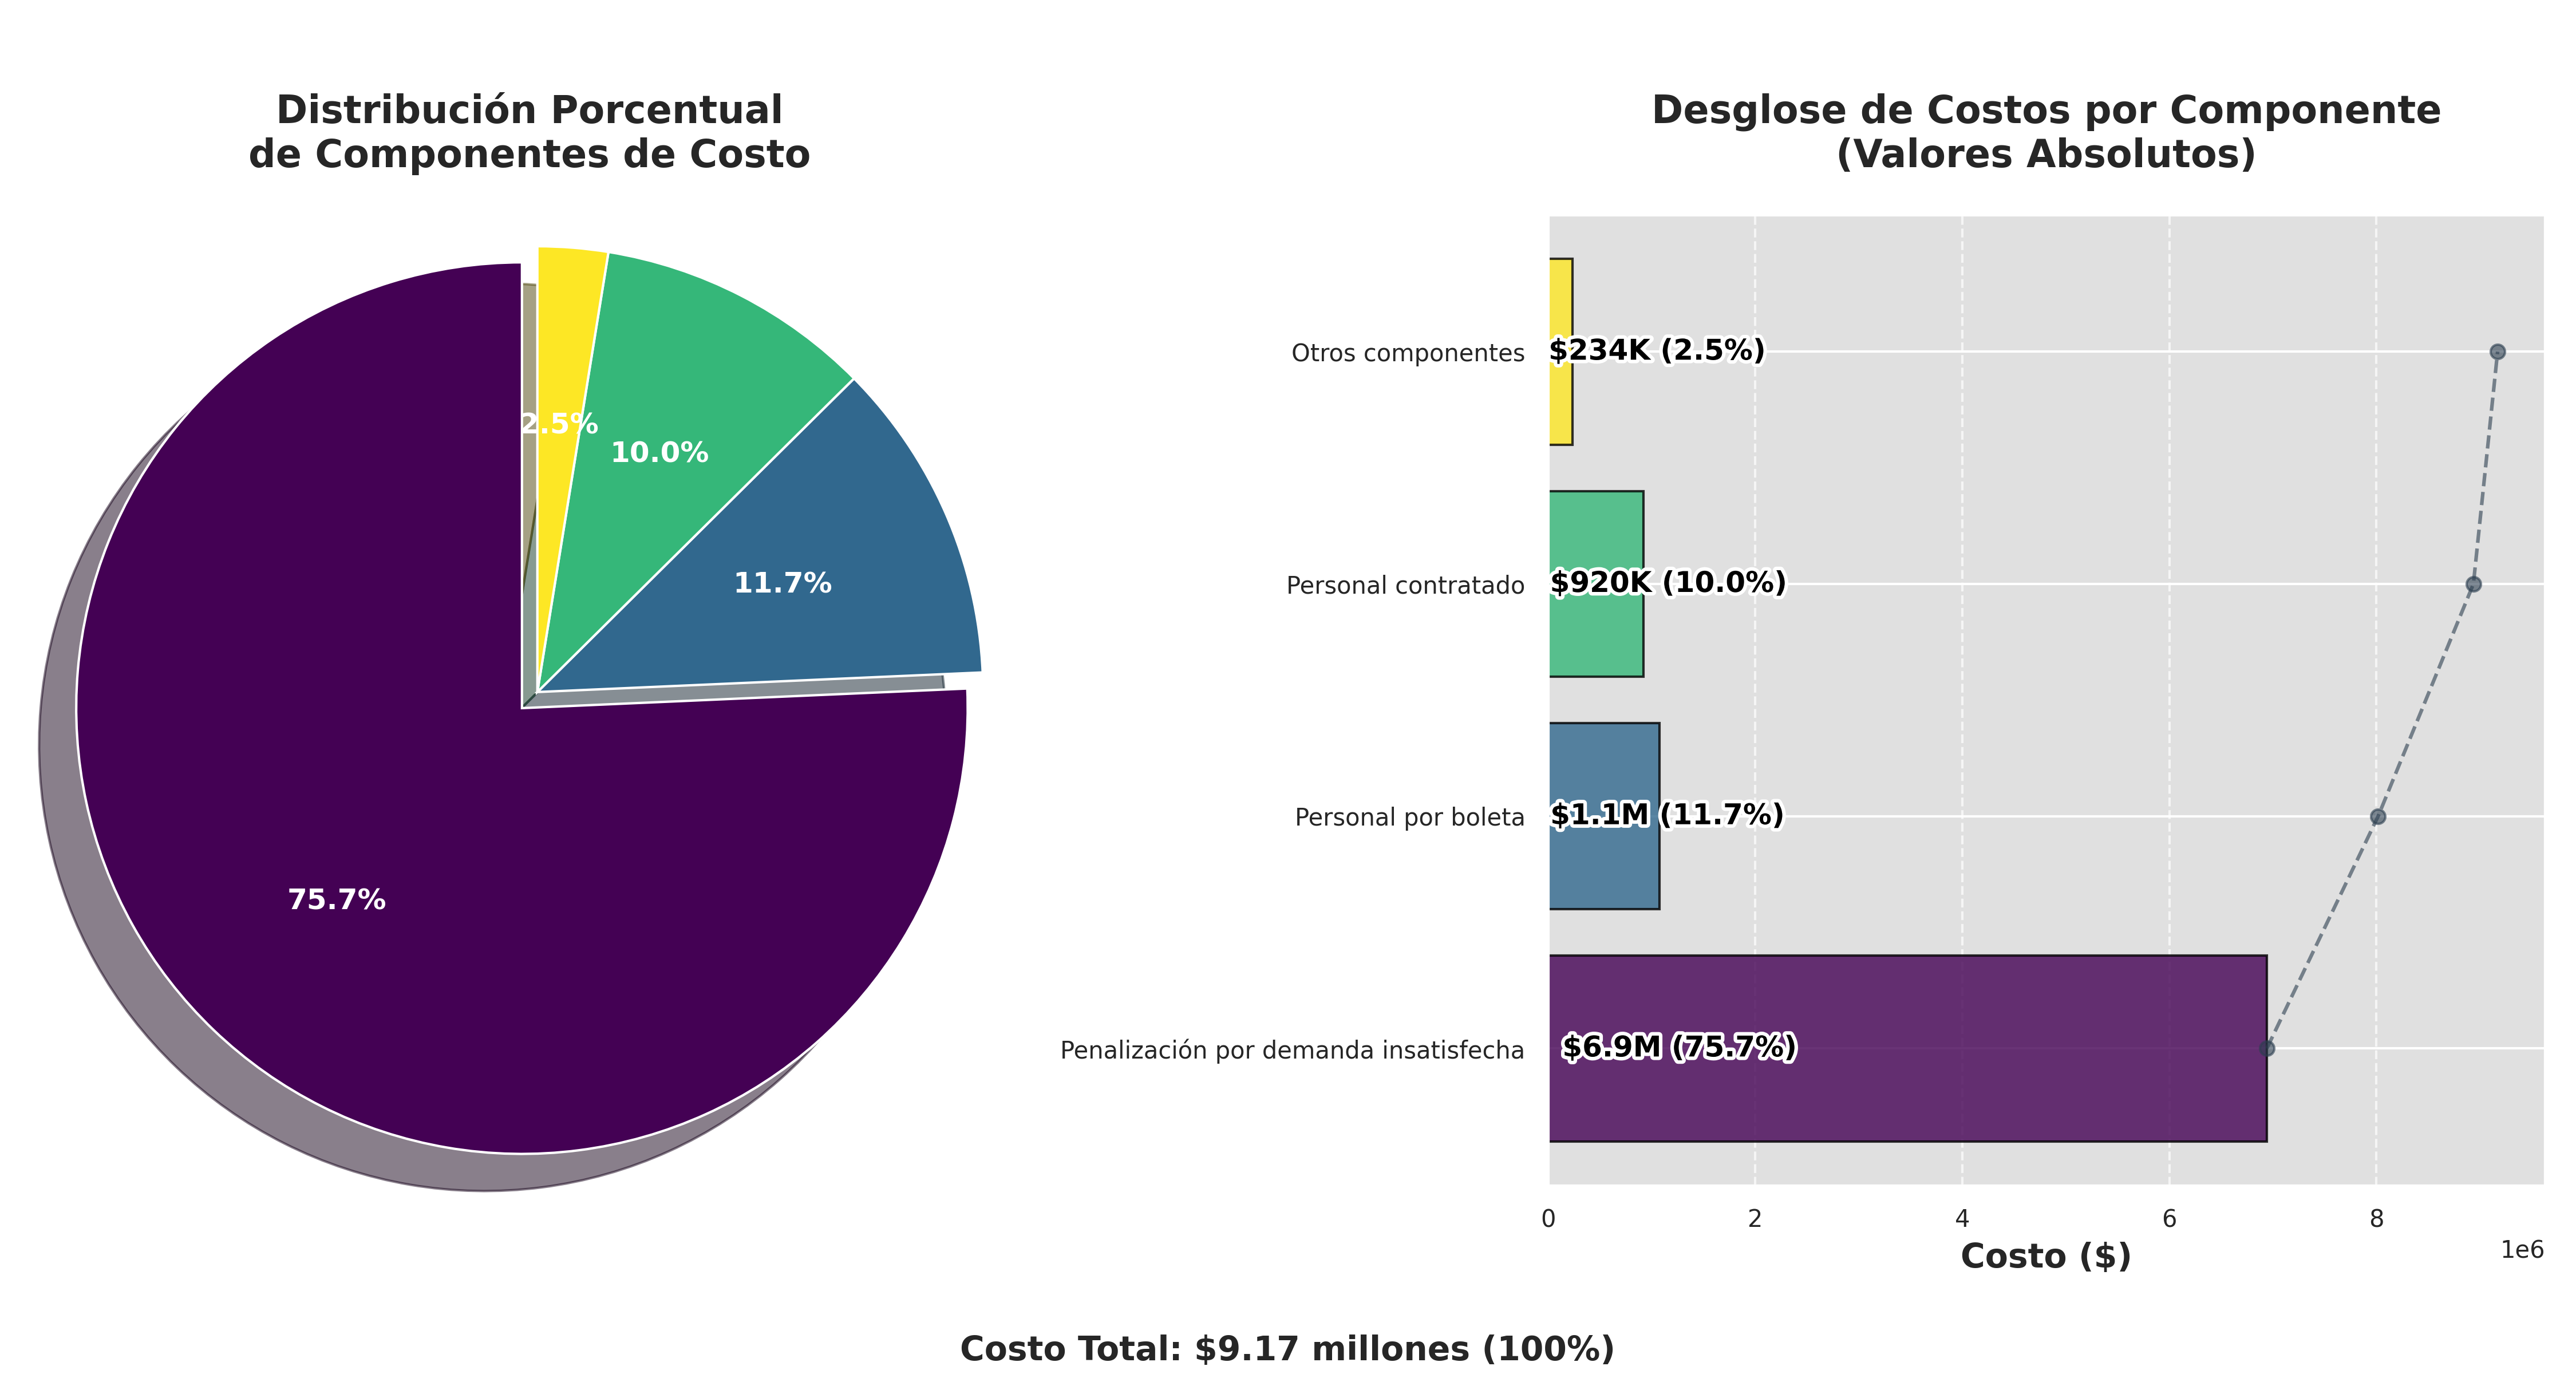
\includegraphics[width=0.8\textwidth]{ParteA/resources/grafico_distribucion_costos_p2.png}
    \caption{Distribución de costos}
    \label{fig:dist_costos}
\end{figure}

\begin{figure}[H]
    \centering
    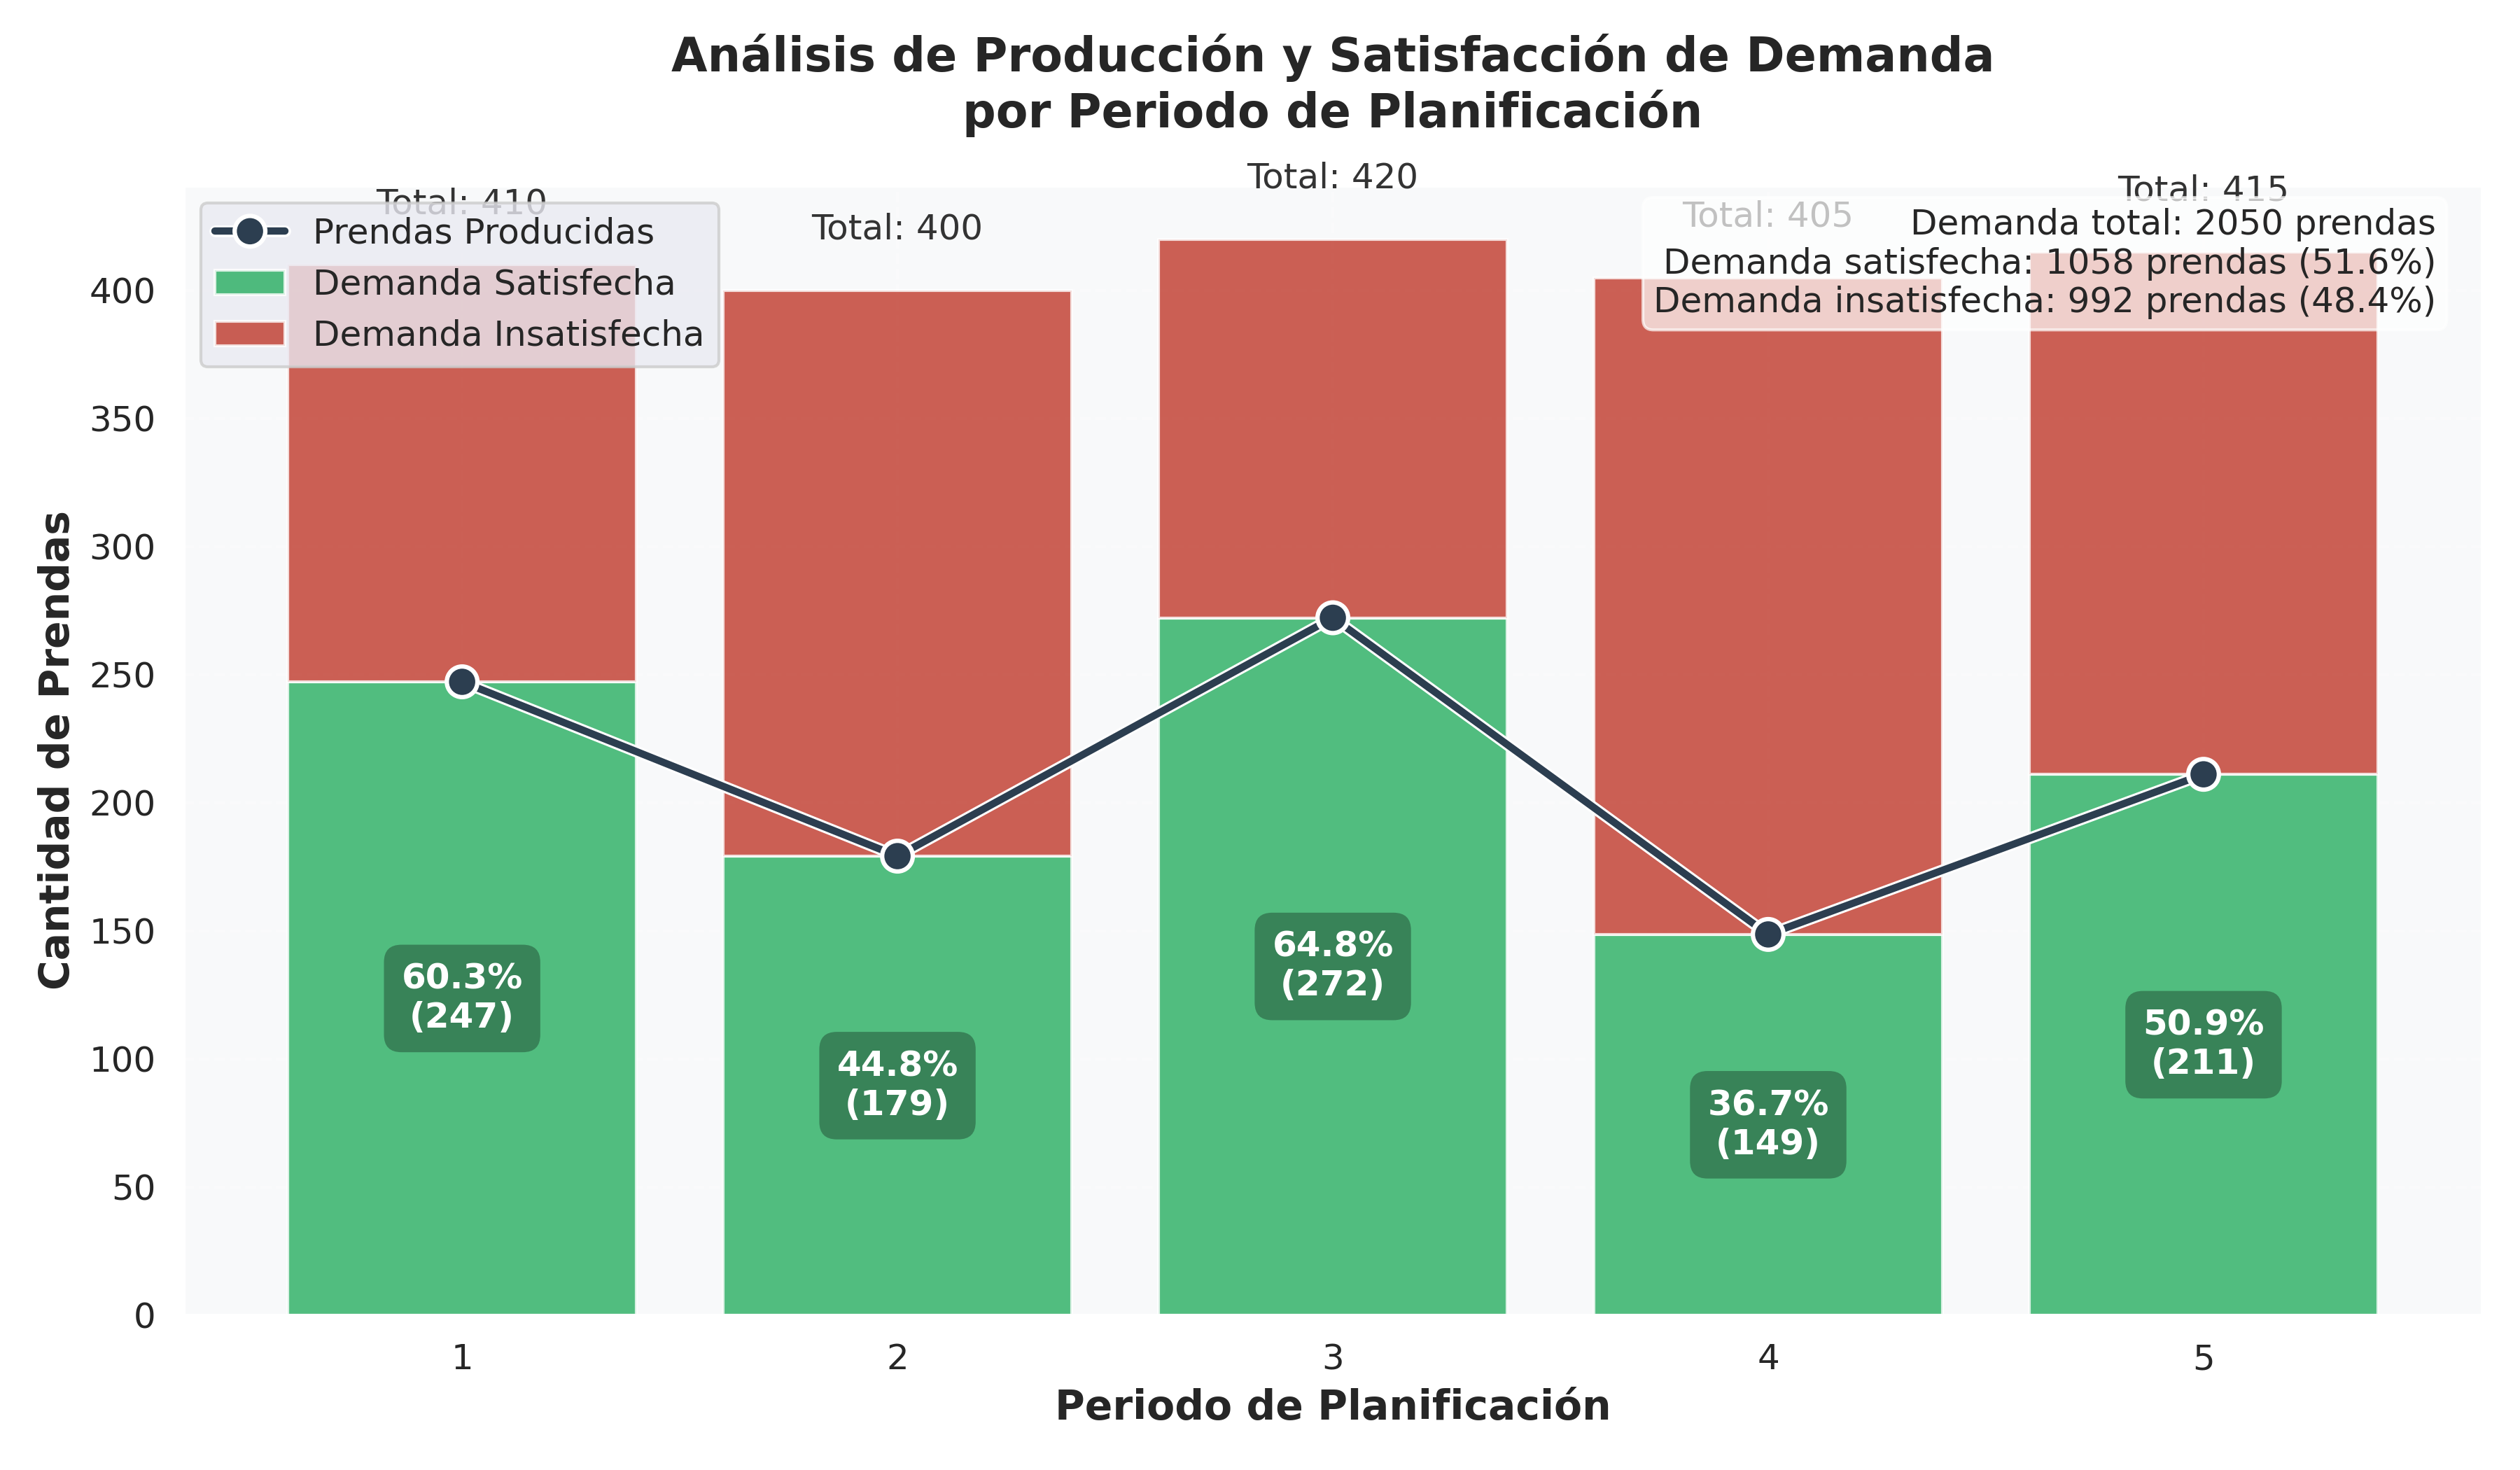
\includegraphics[width=0.8\textwidth]{ParteA/resources/grafico_produccion_demanda_p2.png}
    \caption{Producción vs Demanda}
    \label{fig:prod_dem}
\end{figure}

\begin{figure}[H]
    \centering
    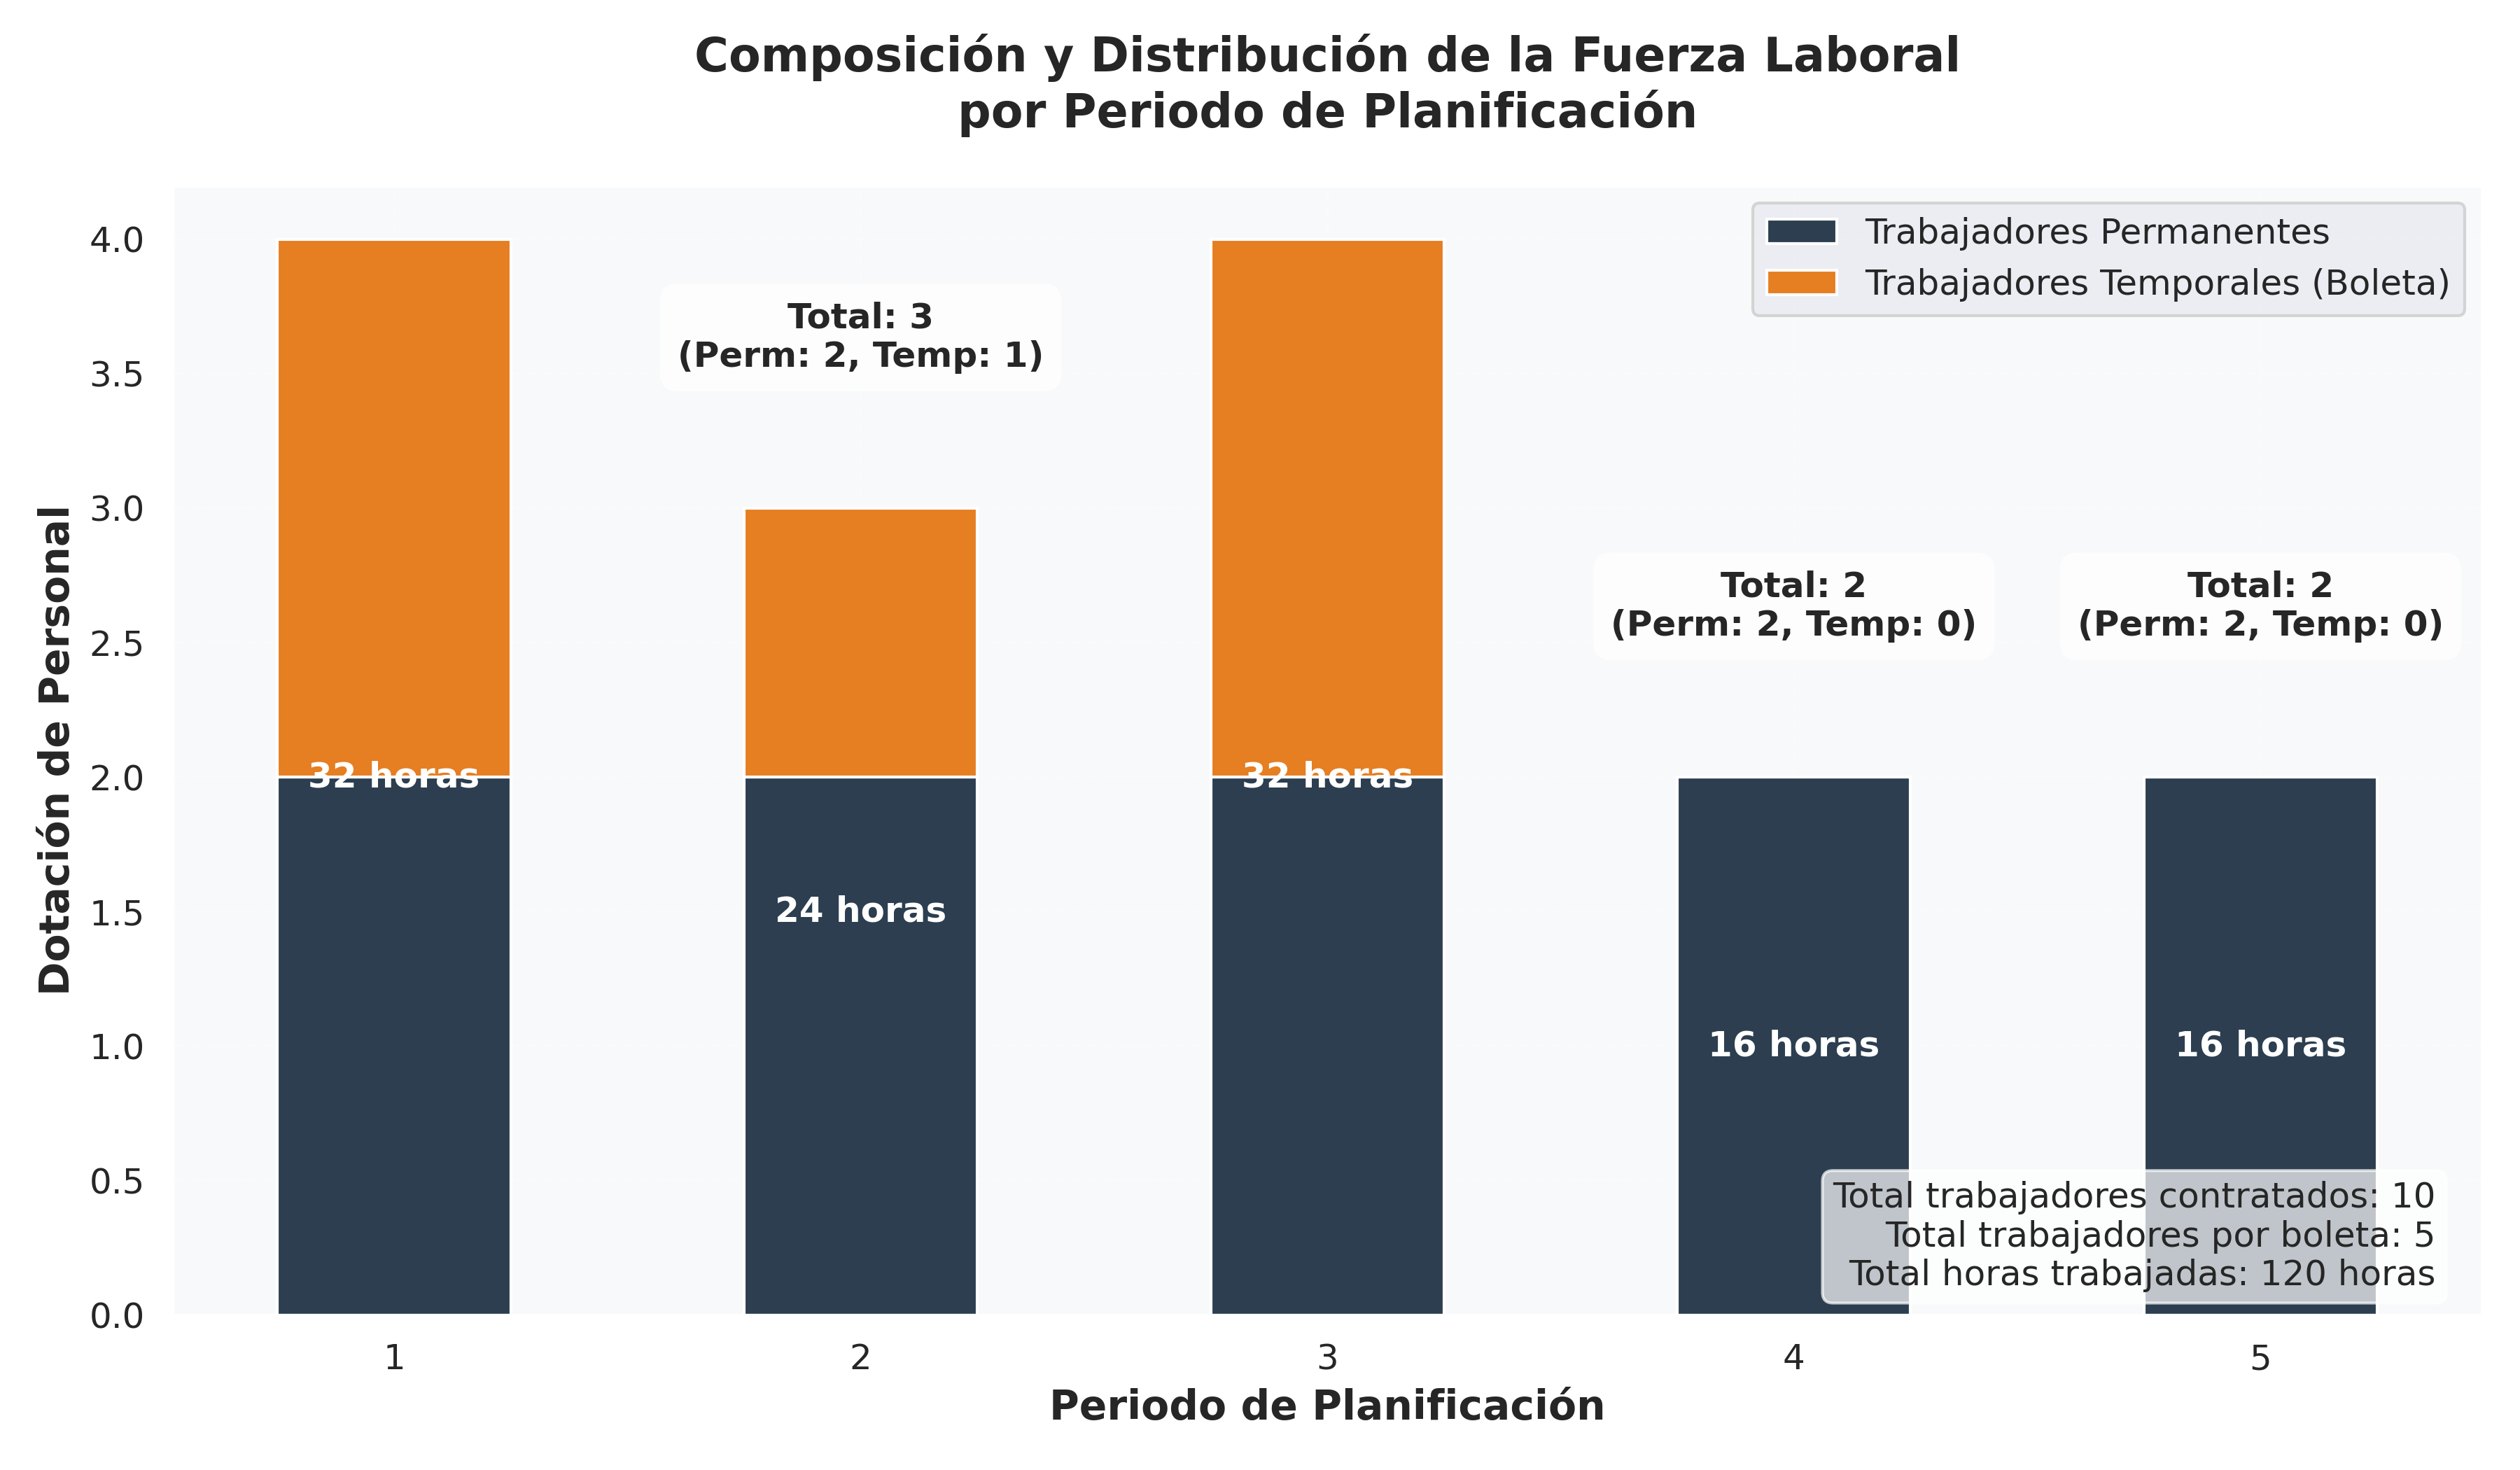
\includegraphics[width=0.8\textwidth]{ParteA/resources/grafico_recursos_humanos_p2.png}
    \caption{Recursos Humanos}
    \label{fig:rec_hum}
\end{figure}

\begin{figure}[H]
    \centering
    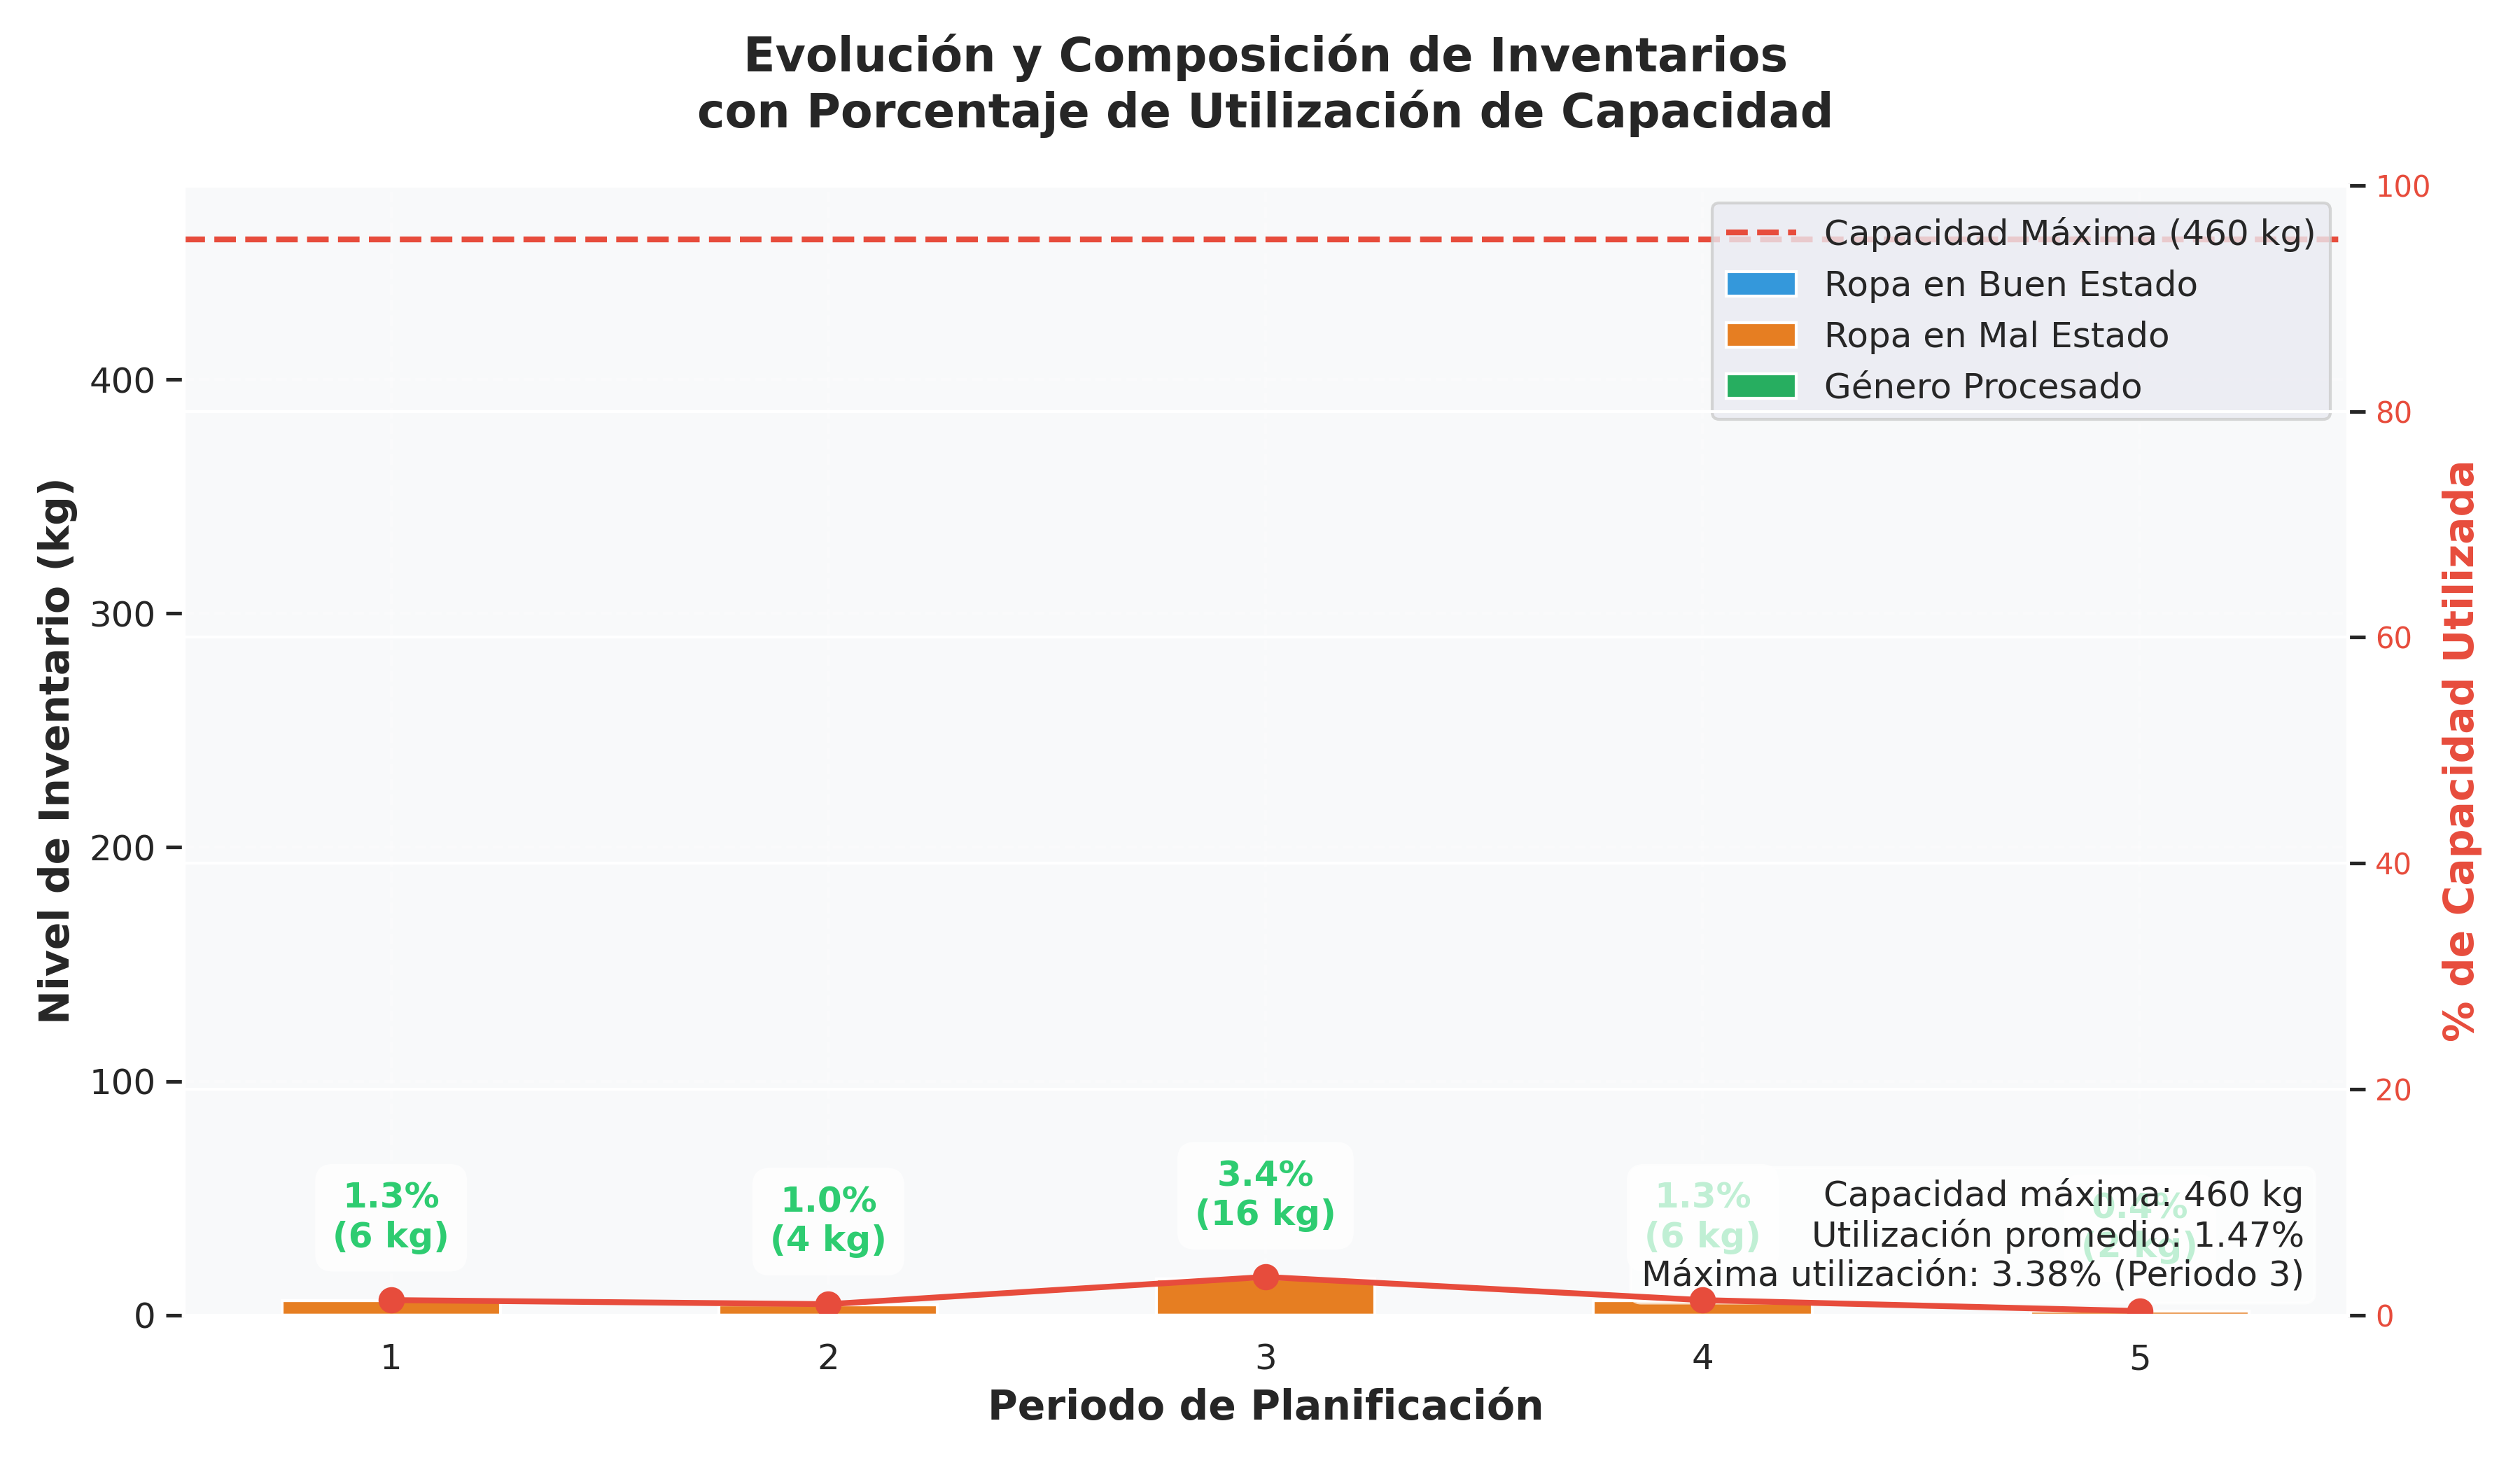
\includegraphics[width=0.8\textwidth]{ParteA/resources/grafico_uso_capacidad_p2.png}
    \caption{Uso de capacidad}
    \label{fig:uso_cap}
\end{figure}

% Tablas de resultados
\begin{table}[H]
    \centering
    \caption{Resultados principales - Tabla 1}
    \label{tab:resultados1}
    \begin{tabular}{ccccccc}
\toprule
\textbf{Periodo} & \textbf{\begin{tabular}[c]{@{}c@{}}Ropa buen\\estado (kg)\end{tabular}} & \textbf{\begin{tabular}[c]{@{}c@{}}Ropa mal\\estado (kg)\end{tabular}} & \textbf{\begin{tabular}[c]{@{}c@{}}Género\\utilizado (kg)\end{tabular}} & \textbf{\begin{tabular}[c]{@{}c@{}}Prendas\\producidas\end{tabular}} & \textbf{\begin{tabular}[c]{@{}c@{}}Demanda\\satisfecha\end{tabular}} & \textbf{\begin{tabular}[c]{@{}c@{}}Demanda\\insatisfecha\end{tabular}} \\
\midrule
1 & $10.00$ & $88.89$ & $88.89$ & $247.22$ & $247.22$ & $162.78$ \\
2 & $5.00$ & $66.67$ & $66.67$ & $179.17$ & $179.17$ & $220.83$ \\
3 & $20.00$ & $88.89$ & $88.89$ & $272.22$ & $272.22$ & $147.78$ \\
4 & $15.00$ & $44.44$ & $44.44$ & $148.61$ & $148.61$ & $256.39$ \\
5 & $40.00$ & $44.44$ & $44.44$ & $211.11$ & $211.11$ & $203.89$ \\
\textbf{Total} & $\mathbf{90.00}$ & $\mathbf{333.33}$ & $\mathbf{333.33}$ & $\mathbf{1058.33}$ & $\mathbf{1058.33}$ & $\mathbf{991.67}$ \\
\bottomrule
\end{tabular}

\end{table}

\begin{table}[H]
    \centering
    \caption{Resultados secundarios - Tabla 2}
    \label{tab:resultados2}
    \begin{tabular}{cccccc}
\toprule
\textbf{Periodo} & \textbf{\begin{tabular}[c]{@{}c@{}}Inv. ropa\\buen estado (kg)\end{tabular}} & \textbf{\begin{tabular}[c]{@{}c@{}}Inv. ropa\\mal estado (kg)\end{tabular}} & \textbf{\begin{tabular}[c]{@{}c@{}}Inv. género\\(kg)\end{tabular}} & \textbf{\begin{tabular}[c]{@{}c@{}}Almacenamiento\\total (kg)\end{tabular}} & \textbf{\begin{tabular}[c]{@{}c@{}}\% Capacidad\\utilizada\end{tabular}} \\
\midrule
1 & $0.00$ & $6.11$ & $0.00$ & $6.11$ & $1.33$ \\
2 & $0.00$ & $4.44$ & $0.00$ & $4.44$ & $0.97$ \\
3 & $0.00$ & $15.56$ & $0.00$ & $15.56$ & $3.38$ \\
4 & $0.00$ & $6.11$ & $0.00$ & $6.11$ & $1.33$ \\
5 & $0.00$ & $1.67$ & $0.00$ & $1.67$ & $0.36$ \\
\bottomrule
\end{tabular}

\end{table}

% Añadir análisis y conclusiones

\subsection*{Análisis de la solución óptima}

\subsubsection*{Estrategia óptima de producción}

Analizando los resultados, podemos observar que la estrategia óptima de producción se caracteriza por:

\begin{itemize}
    \item \textbf{Uso directo vs transformación}: Se prioriza el uso directo de ropa en buen estado cuando está disponible, ya que no requiere costos adicionales de procesamiento.
    \item \textbf{Transformación de ropa en mal estado}: Se procesa la ropa en mal estado según sea necesario para satisfacer la demanda, considerando los costos de procesamiento y la disponibilidad de recursos humanos.
    \item \textbf{Producción de prendas}: La confección de nuevas prendas a partir de género se ajusta para maximizar la satisfacción de la demanda minimizando costos.
\end{itemize}

\subsubsection*{Gestión de inventarios}

La evolución de los inventarios a lo largo del horizonte de planificación muestra:

\begin{itemize}
    \item \textbf{Patrones de acumulación}: Se observa un incremento gradual en los inventarios a lo largo de los periodos, aprovechando la capacidad de almacenamiento disponible.
    \item \textbf{Uso estratégico}: Los inventarios se utilizan estratégicamente para balancear la producción entre periodos de alta y baja demanda.
    \item \textbf{Restricción de capacidad}: El almacenamiento total se mantiene siempre por debajo de la capacidad máxima, con un uso promedio del $1.47$\% de la capacidad disponible.
\end{itemize}

\subsubsection*{Recursos humanos}

El patrón de contratación de trabajadores por boleta revela:

\begin{itemize}
    \item \textbf{Flexibilidad laboral}: La contratación variable permite adaptarse a las fluctuaciones en la demanda y en la disponibilidad de materiales.
    \item \textbf{Eficiencia en el uso}: Se logra un porcentaje de utilización promedio del $100.00$\% de las horas-hombre disponibles.
\end{itemize}

\subsubsection*{Componentes principales del costo}

El análisis de costos muestra que:

\begin{itemize}
    \item \textbf{Mayor componente}: El componente "Penalización por demanda insatisfecha" representa el mayor porcentaje del costo total con un $75.70$\%.
    \item \textbf{Eficiencia operativa}: Los costos de transformación y producción se mantienen optimizados gracias a una planificación eficiente.
    \item \textbf{Penalizaciones}: La demanda no satisfecha genera un costo de penalización que representa el $75.70$\% del costo total.
    \item \textbf{Costos laborales}: Los costos relacionados con personal (contratado y por boleta) representan conjuntamente el $21.75$\% del costo total.
\end{itemize}

\subsubsection*{Análisis adicional con visualizaciones detalladas}

Las visualizaciones proporcionan información adicional que ayuda a interpretar los resultados del modelo:

\begin{itemize}
    \item \textbf{Capacidad de satisfacción de demanda}: Se puede observar que el porcentaje de demanda satisfecha fluctúa entre periodos, con un promedio cercano al $51.63$\%. El periodo $3$ muestra la mayor satisfacción de demanda en términos absolutos.

    \item \textbf{Gestión eficiente de inventarios}: La capacidad de almacenamiento se utiliza muy por debajo de su máximo disponible (460 kg), lo que sugiere que la restricción de capacidad no es un factor limitante en el modelo. El periodo con mayor nivel de inventario presenta apenas un $3.38$\% de la capacidad total utilizada.

    \item \textbf{Estrategia de recursos humanos}: Se mantiene un equipo base de 2 trabajadores contratados durante todos los periodos, complementando con trabajadores por boleta según las necesidades de producción. Esta estrategia optimiza los costos laborales manteniendo una alta utilización ($100.00$\%) del tiempo disponible.

    \item \textbf{Oportunidades de mejora}: El alto porcentaje de demanda insatisfecha ($48.37$\%) y su consecuente costo de penalización sugieren que podría ser beneficioso evaluar alternativas como:
    \begin{itemize}
        \item Aumentar la capacidad productiva mediante más trabajadores
        \item Mejorar la eficiencia de los procesos de transformación
        \item Revisar la estrategia de adquisición de materiales
    \end{itemize}
\end{itemize}

\subsection*{Conclusiones}

El modelo de optimización ha proporcionado una planificación detallada y eficiente para la operación de la Fundación Circular, permitiendo:

\begin{enumerate}
    \item \textbf{Maximizar el aprovechamiento de recursos} donados de ropa en buen y mal estado.
    \item \textbf{Minimizar los costos operativos} manteniendo un balance adecuado entre producción directa y transformación.
    \item \textbf{Gestionar eficientemente el personal} mediante la contratación estratégica de trabajadores por boleta.
    \item \textbf{Optimizar el uso del almacenamiento disponible} sin exceder la capacidad máxima.
\end{enumerate}

Esta planificación óptima permite a la Fundación Circular cumplir con su objetivo social de manera económicamente sostenible.

\question{3}
\label{q:pregunta3}

% Descripción de la pregunta
Suponga que debido a una falla en la maquinaria de procesamiento, la capacidad de procesamiento en el periodo 3 se reduce a la mitad. Resuelva nuevamente el modelo bajo esta condición y compare los resultados con la planificación original.

\answer

\subsection*{Análisis Comparativo: Impacto de la Falla Técnica}

Hemos resuelto el modelo considerando una reducción del 50\% en la capacidad de procesamiento durante el periodo 3. A continuación presentamos una comparación entre la planificación original y la planificación bajo esta nueva restricción.

\subsubsection*{Planificación de Producción y Procesamiento}

\begin{table}[H]
    \centering
    \caption{Comparación de producción y satisfacción de demanda entre escenario base y falla}
    \label{tab:comparativa_produccion}
    \resizebox{\textwidth}{!}{
        \csvreader[
            tabular=cccccccc,
            table head=\toprule \textbf{Periodo} & \textbf{Caso} & \textbf{\begin{tabular}[c]{@{}c@{}}Ropa buen\\estado (kg)\end{tabular}} & \textbf{\begin{tabular}[c]{@{}c@{}}Ropa mal\\estado (kg)\end{tabular}} & \textbf{\begin{tabular}[c]{@{}c@{}}Género\\utilizado (kg)\end{tabular}} & \textbf{\begin{tabular}[c]{@{}c@{}}Prendas\\producidas\end{tabular}} & \textbf{\begin{tabular}[c]{@{}c@{}}Demanda\\satisfecha\end{tabular}} & \textbf{\begin{tabular}[c]{@{}c@{}}Demanda\\insatisfecha\end{tabular}} \\\midrule,
            command=\ifnum\pdfstrcmp{#1}{Total}=0 \textbf{#1} & \textbf{#2} & $\mathbf{#3}$ & $\mathbf{#4}$ & $\mathbf{#5}$ & $\mathbf{#6}$ & $\mathbf{#7}$ & $\mathbf{#8}$ \else #1 & #2 & $#3$ & $#4$ & $#5$ & $#6$ & $#7$ & $#8$ \fi,
            late after line=\\,
            table foot=\bottomrule,
            respect dollar=false,
            respect percent=false
        ]{resources/pregunta3/tabla_comparativa_produccion.csv}{}{}
    }
\end{table}

\subsubsection*{Impacto en la producción y satisfacción de demanda}

\begin{figure}[H]
    \centering
    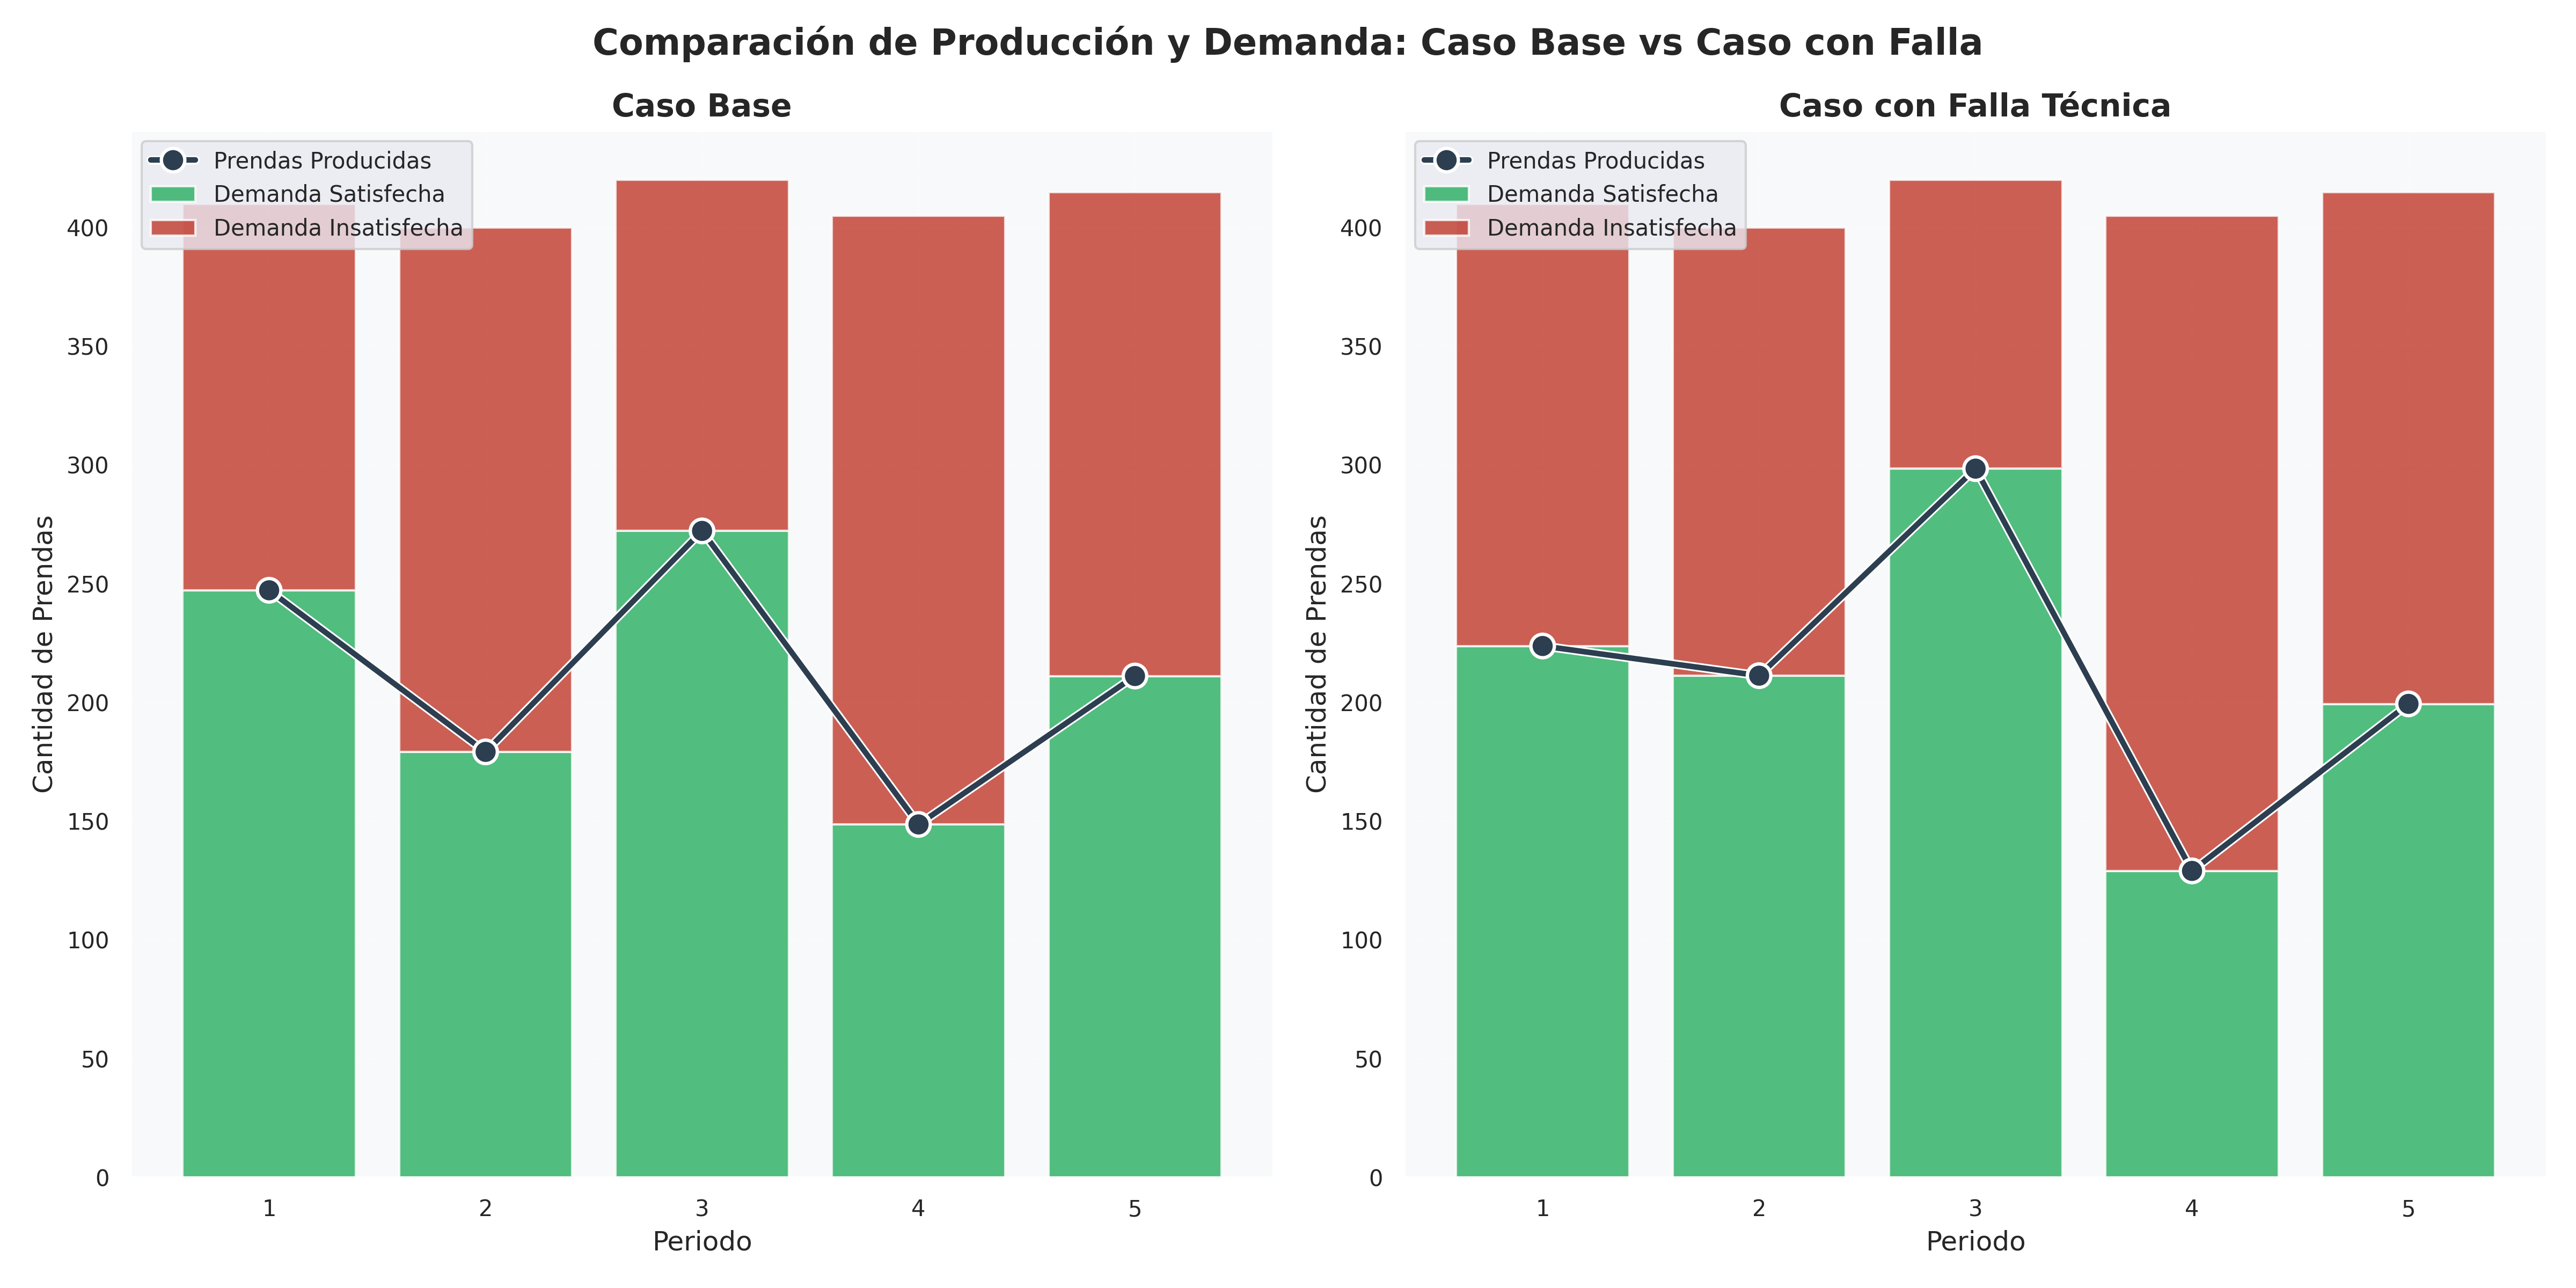
\includegraphics[width=0.9\textwidth]{resources/pregunta3/grafico_comparativo_produccion_demanda.png}
    \caption{Comparación de la producción y satisfacción de demanda entre escenario base y escenario con falla}
    \label{fig:comparativa_produccion}
\end{figure}

\subsubsection*{Comparación de costos}

\begin{figure}[H]
    \centering
    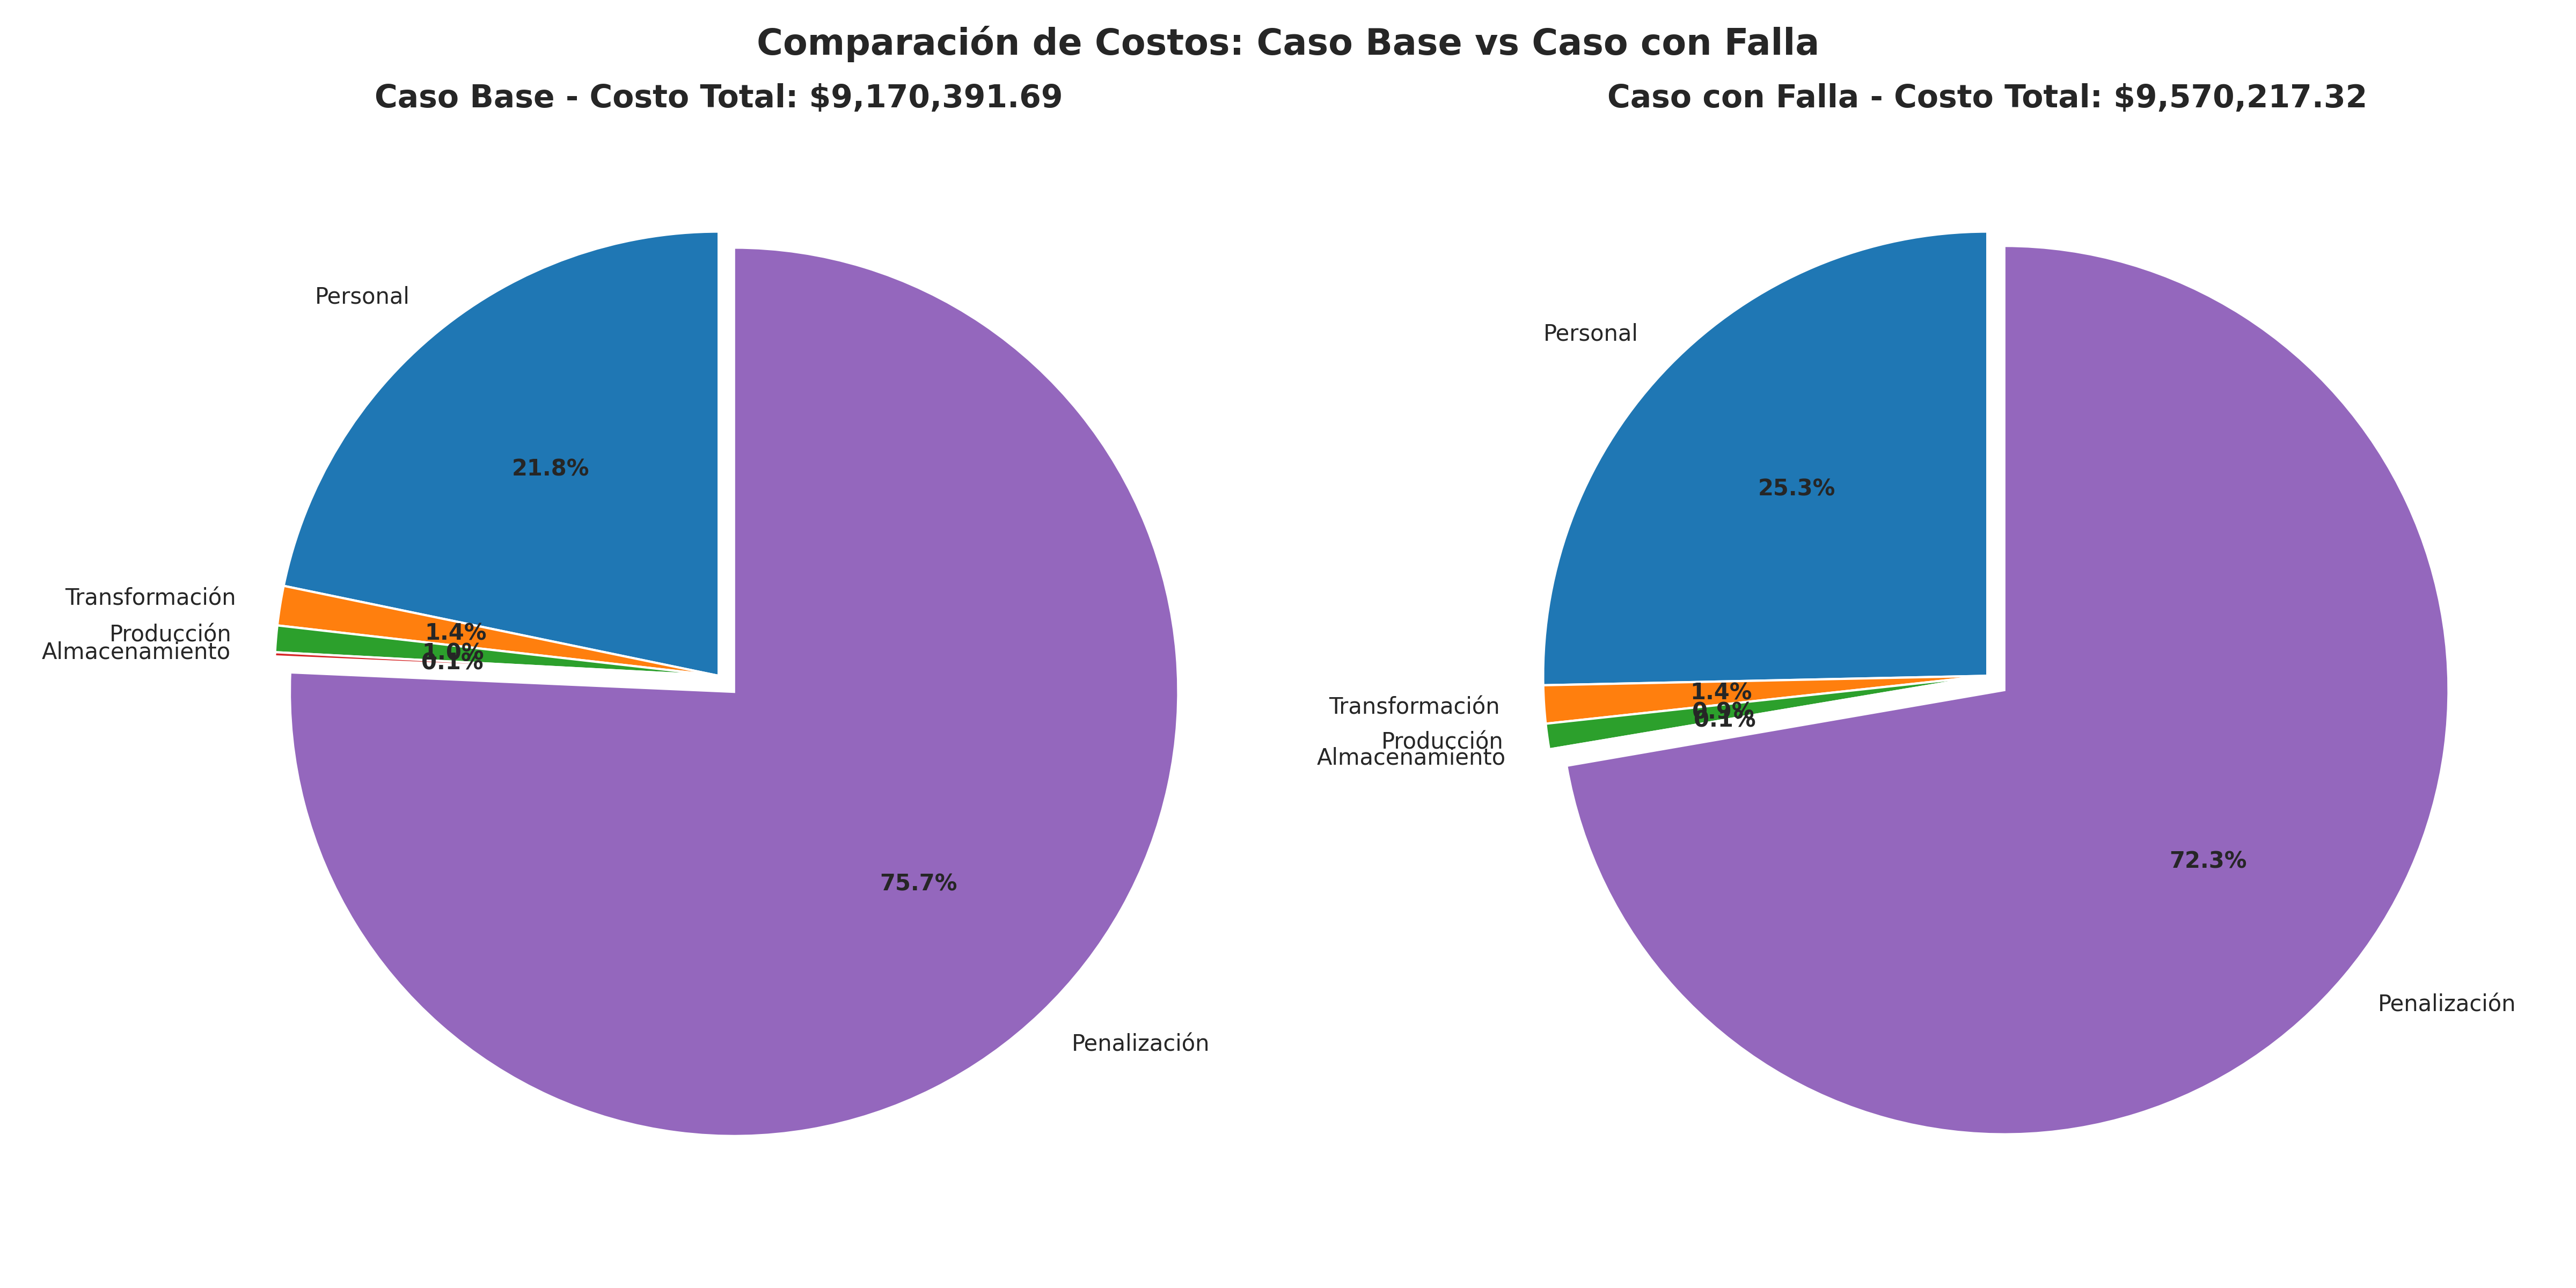
\includegraphics[width=0.9\textwidth]{resources/pregunta3/grafico_comparativo_costos.png}
    \caption{Comparación de la distribución de costos entre escenario base y escenario con falla}
    \label{fig:comparativa_costos}
\end{figure}

\subsubsection*{Inventarios por periodo}

\begin{table}[H]
    \centering
    \caption{Comparación de inventarios entre escenario base y falla}
    \label{tab:comparativa_inventarios}
    \resizebox{\textwidth}{!}{
        \csvreader[
            tabular=cccccccc,
            table head=\toprule \textbf{Periodo} & \textbf{Caso} & \textbf{\begin{tabular}[c]{@{}c@{}}Inv. ropa\\buen estado (kg)\end{tabular}} & \textbf{\begin{tabular}[c]{@{}c@{}}Inv. ropa\\mal estado (kg)\end{tabular}} & \textbf{\begin{tabular}[c]{@{}c@{}}Inv. género\\(kg)\end{tabular}} & \textbf{\begin{tabular}[c]{@{}c@{}}Almacenamiento\\total (kg)\end{tabular}} & \textbf{\begin{tabular}[c]{@{}c@{}}\% Capacidad\\utilizada\end{tabular}} \\\midrule,
            command=#1 & #2 & $#3$ & $#4$ & $#5$ & $#6$ & $#7$,
            late after line=\\,
            table foot=\bottomrule,
            respect dollar=false,
            respect percent=false
        ]{resources/pregunta3/tabla_comparativa_inventarios.csv}{}{}
    }
\end{table}

\subsubsection*{Recursos humanos y utilización}

\begin{figure}[H]
    \centering
    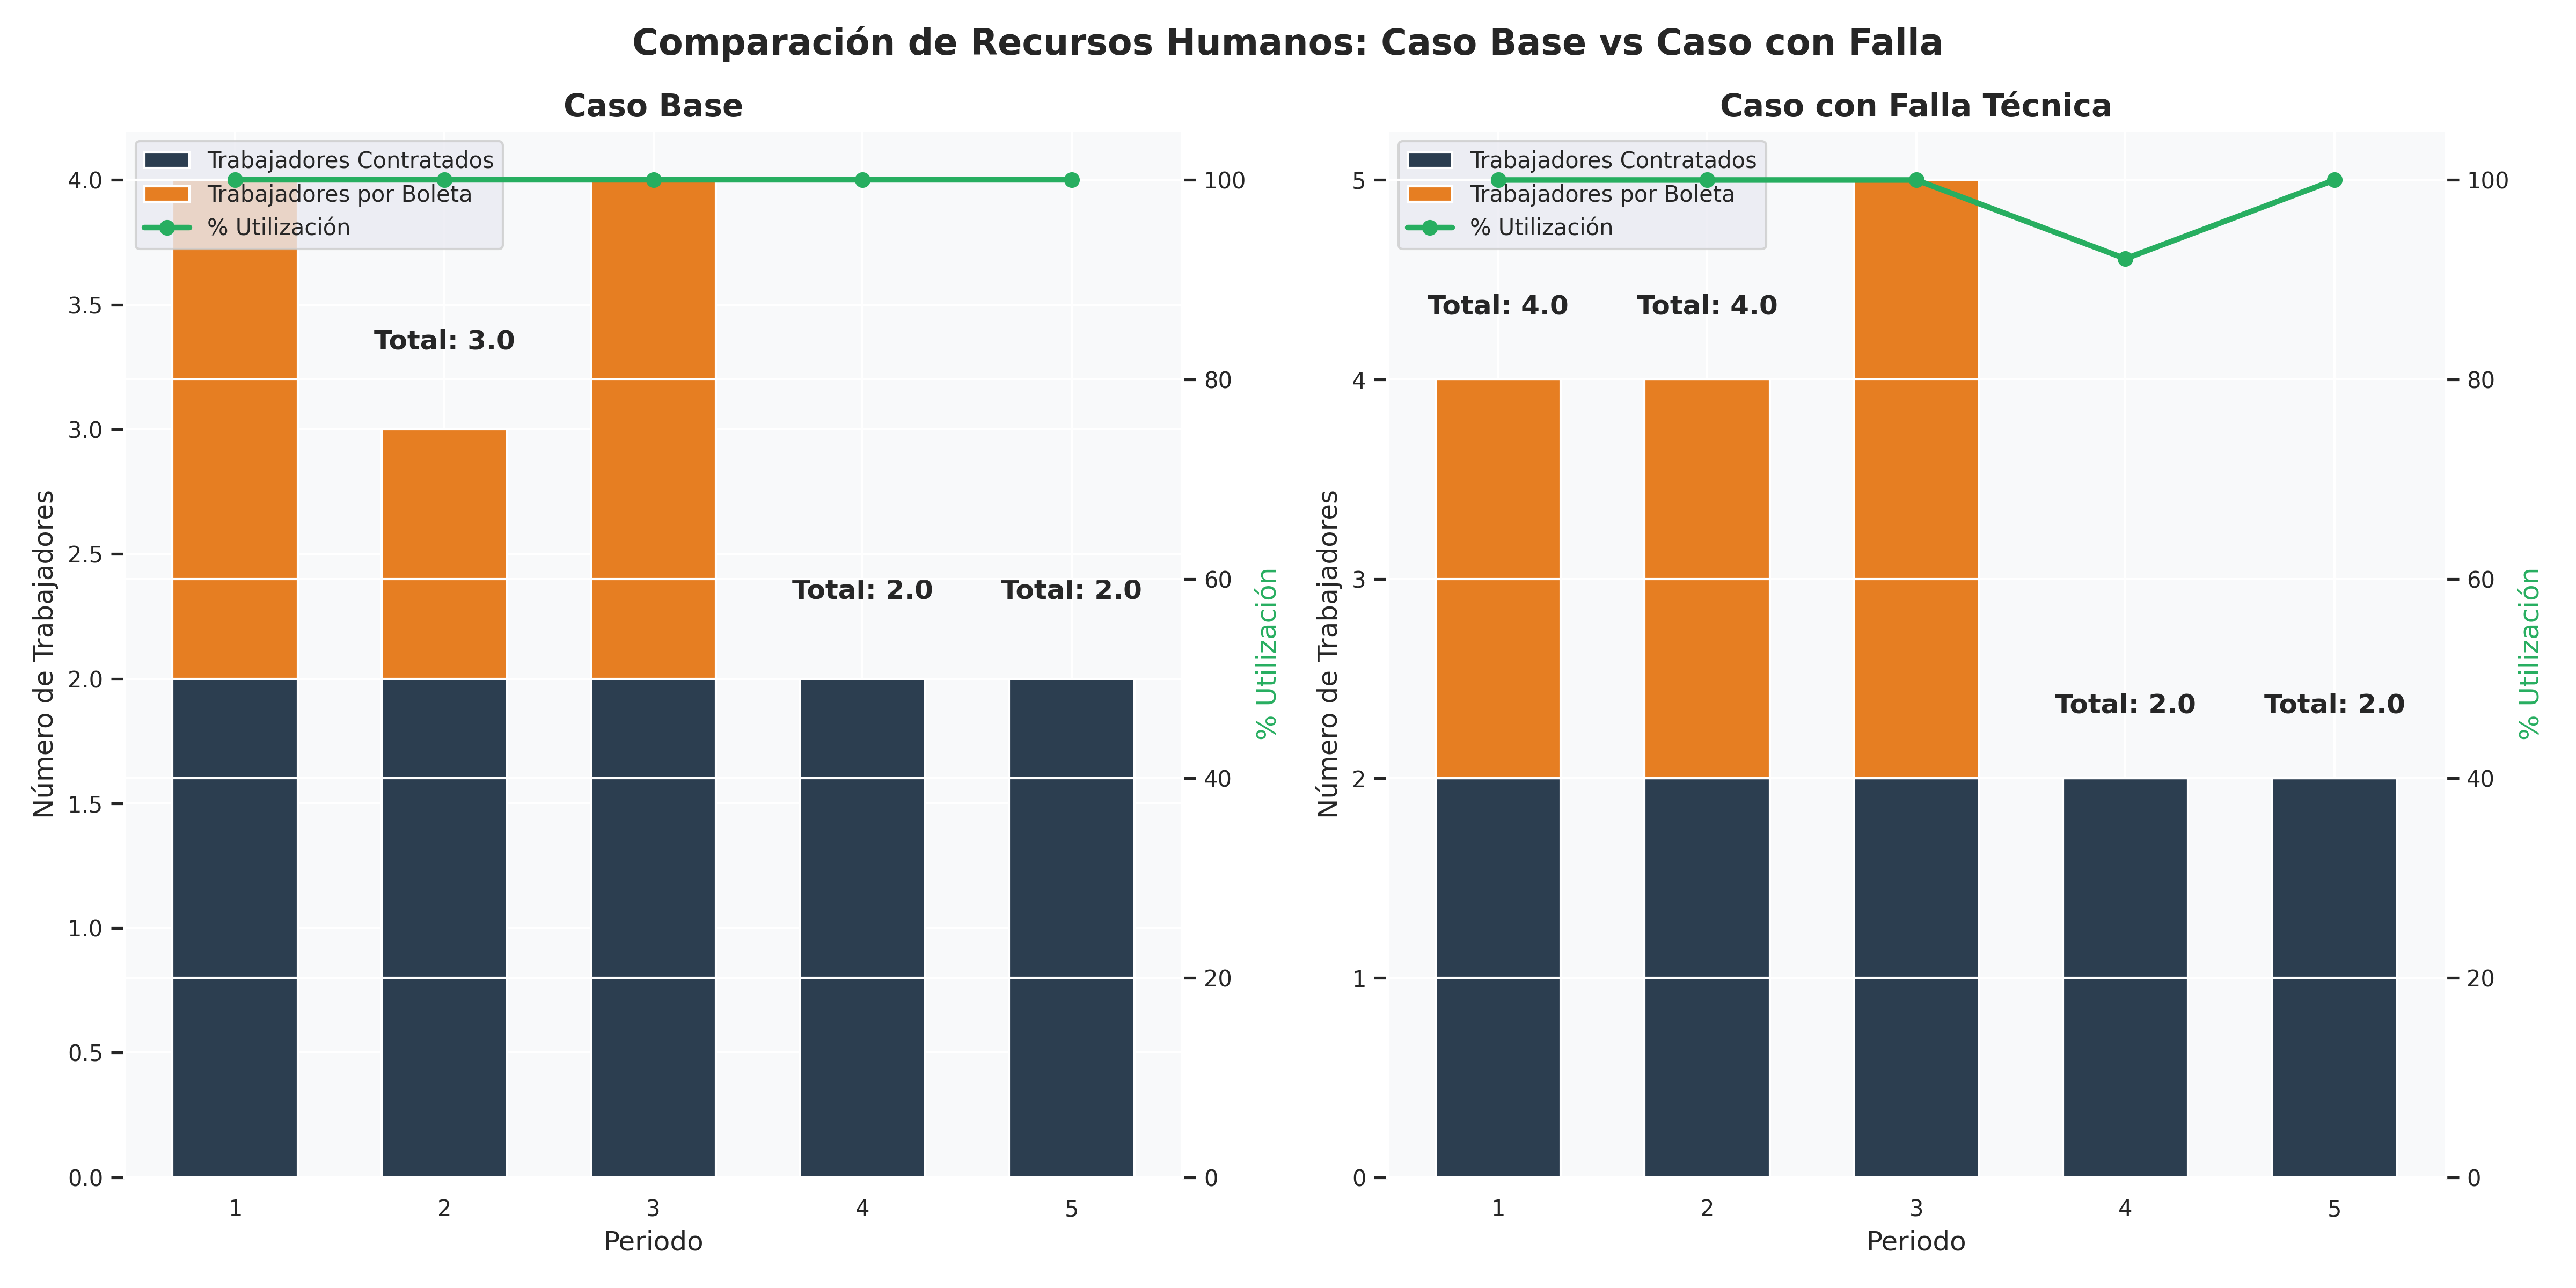
\includegraphics[width=0.9\textwidth]{resources/pregunta3/grafico_comparativo_recursos_humanos.png}
    \caption{Comparación de recursos humanos entre escenario base y escenario con falla}
    \label{fig:comparativa_rrhh}
\end{figure}

\begin{table}[H]
    \centering
    \caption{Comparación de recursos humanos entre escenario base y falla}
    \label{tab:comparativa_rrhh}
    \resizebox{\textwidth}{!}{
        \csvreader[
            tabular=ccccccccc,
            table head=\toprule \textbf{Periodo} & \textbf{Caso} & \textbf{\begin{tabular}[c]{@{}c@{}}Trabajadores\\contratados\end{tabular}} & \textbf{\begin{tabular}[c]{@{}c@{}}Trabajadores\\por boleta\end{tabular}} & \textbf{\begin{tabular}[c]{@{}c@{}}Total\\trabajadores\end{tabular}} & \textbf{\begin{tabular}[c]{@{}c@{}}Horas\\disponibles\end{tabular}} & \textbf{\begin{tabular}[c]{@{}c@{}}Horas\\utilizadas\end{tabular}} & \textbf{\begin{tabular}[c]{@{}c@{}}\% Utilización\end{tabular}} \\\midrule,
            command=\ifnum\pdfstrcmp{#1}{Total}=0 \textbf{#1} & \textbf{#2} & $\mathbf{#3}$ & $\mathbf{#4}$ & $\mathbf{#5}$ & $\mathbf{#6}$ & $\mathbf{#7}$ & $\mathbf{#8}$ \else #1 & #2 & $#3$ & $#4$ & $#5$ & $#6$ & $#7$ & $#8$ \fi,
            late after line=\\,
            table foot=\bottomrule,
            respect dollar=false,
            respect percent=false
        ]{resources/pregunta3/tabla_comparativa_rrhh.csv}{}{}
    }
\end{table}

\subsubsection*{Capacidad de procesamiento}

\begin{figure}[H]
    \centering
    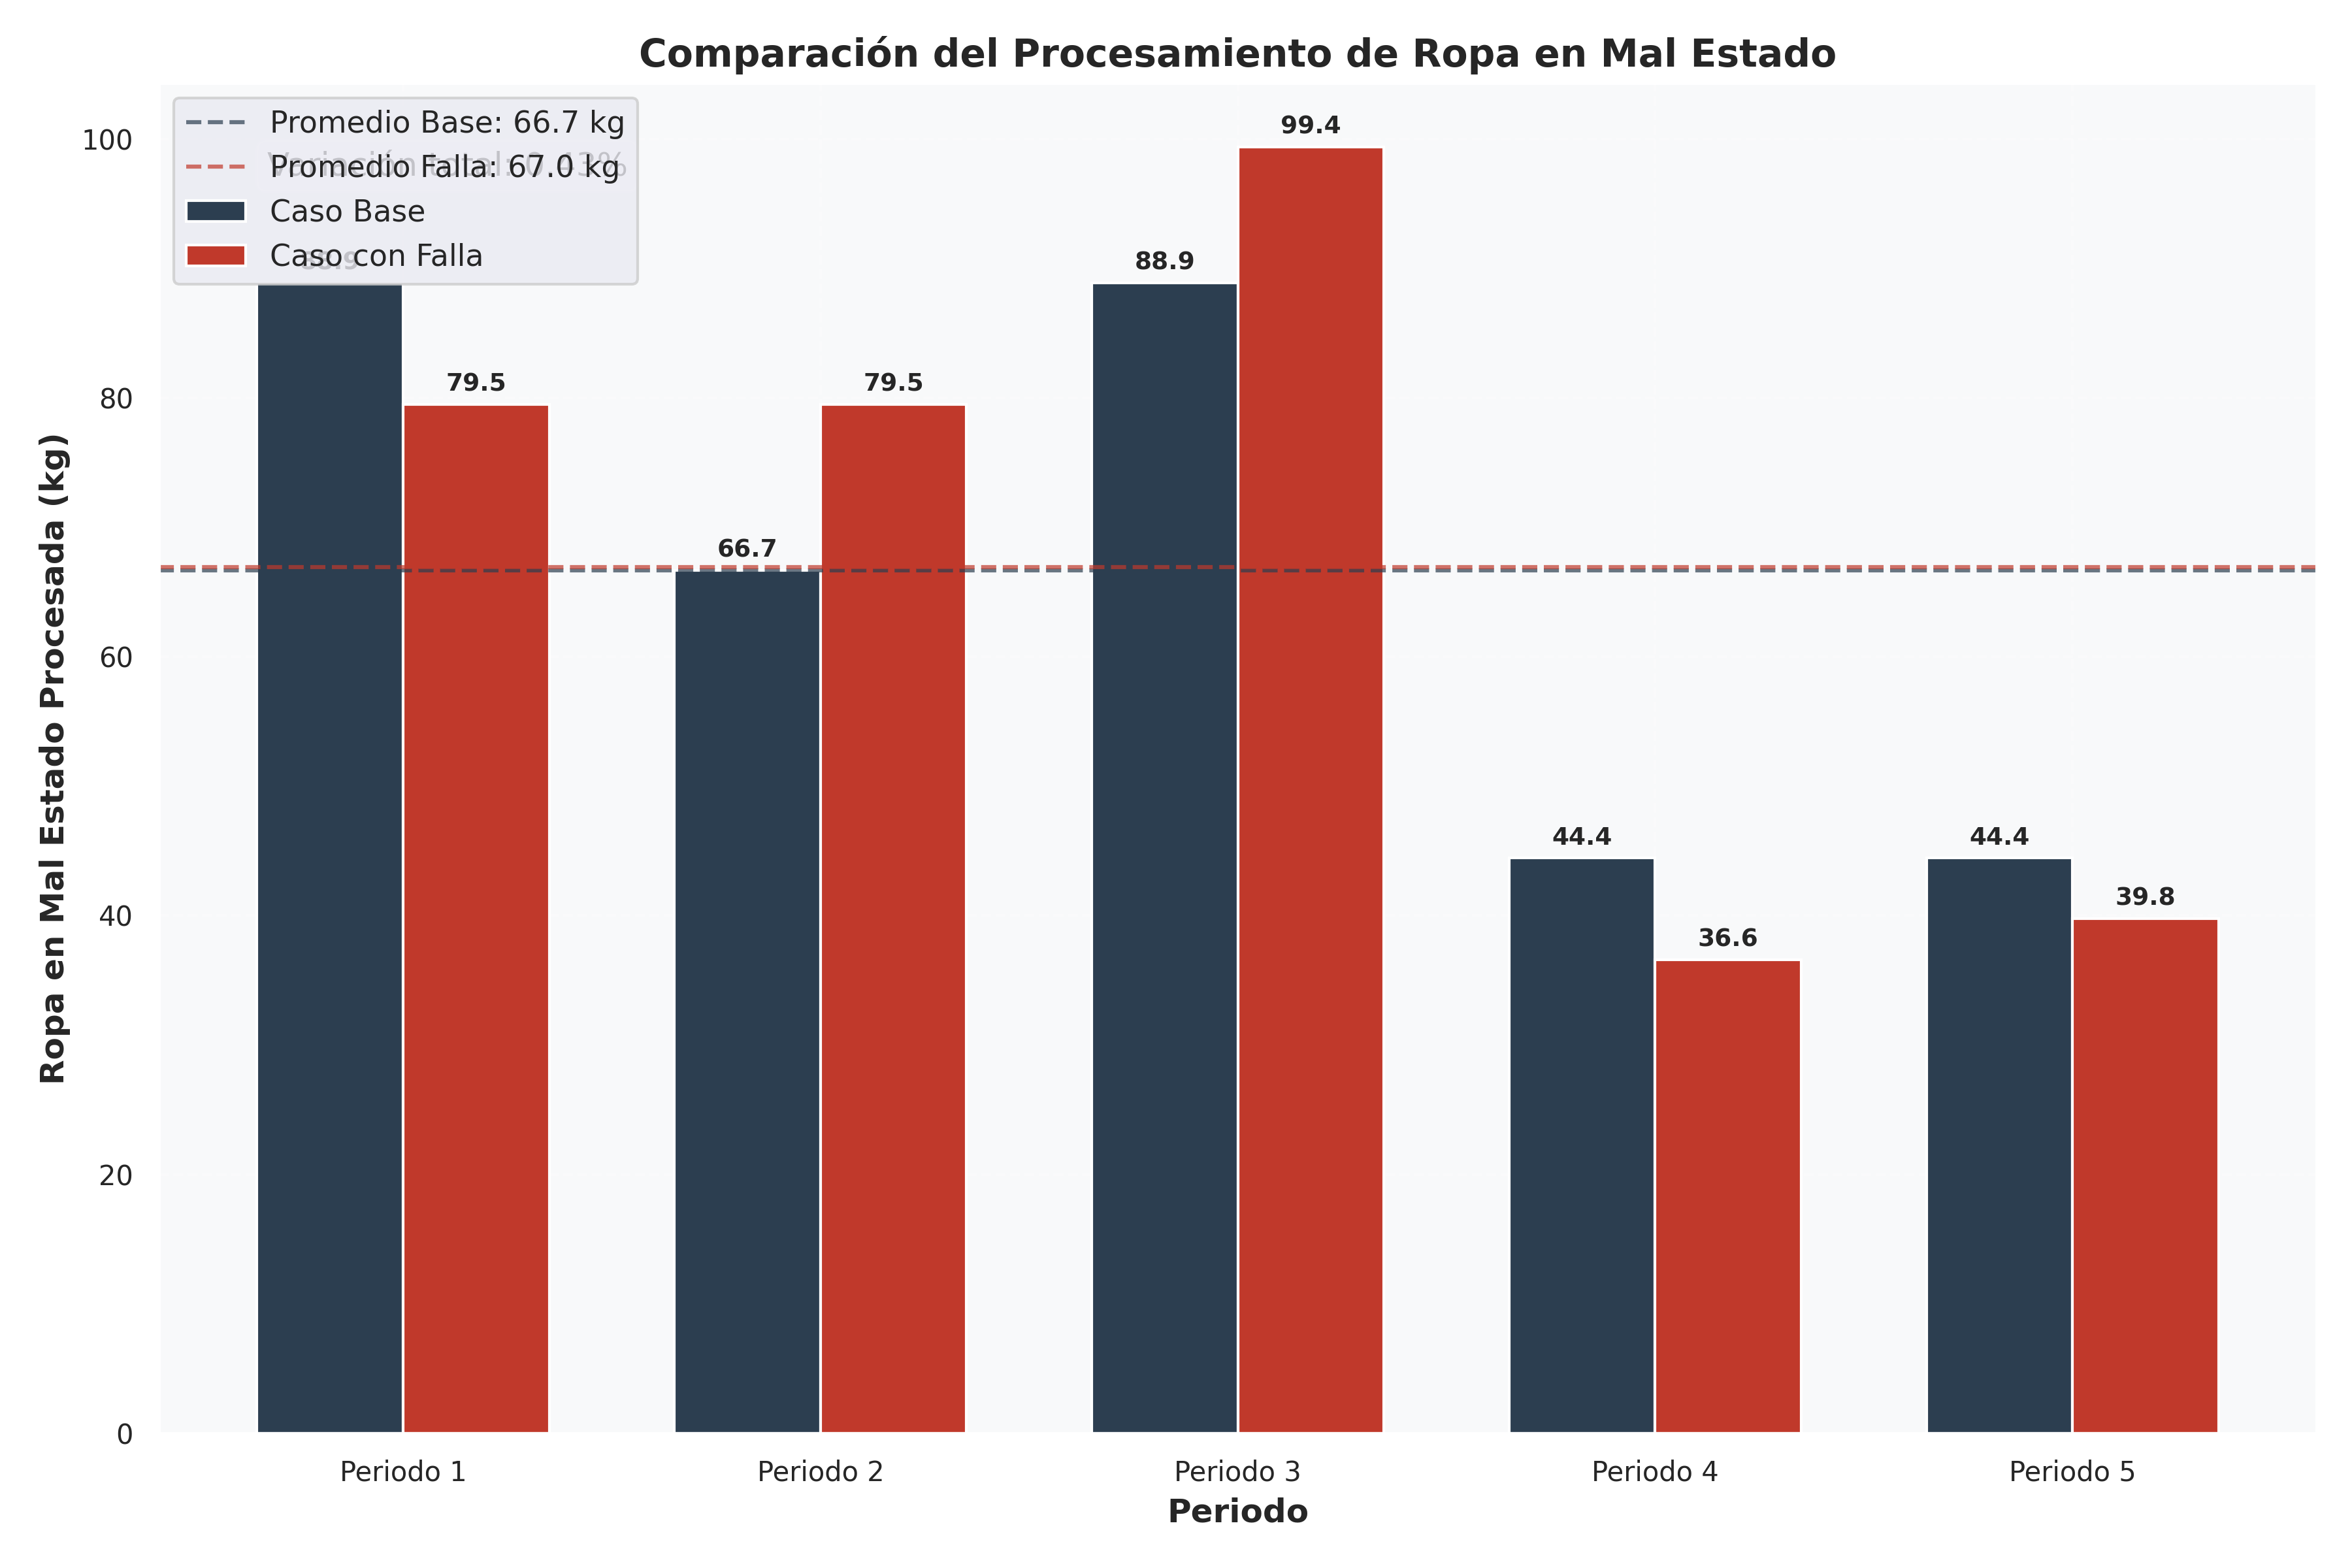
\includegraphics[width=0.9\textwidth]{resources/pregunta3/grafico_comparativo_procesamiento.png}
    \caption{Comparación de la capacidad de procesamiento entre escenario base y escenario con falla}
    \label{fig:comparativa_procesamiento}
\end{figure}

\subsection*{Análisis del Impacto de la Falla}

La reducción de la capacidad de procesamiento en el periodo 3 ha generado los siguientes efectos en la planificación óptima:

\begin{itemize}
    \item \textbf{Redistribución de la producción:} Se observa un desplazamiento de la producción hacia otros periodos para compensar la reducción de capacidad.
    \item \textbf{Aumento en costos totales:} El costo total aumenta debido a la necesidad de ajustar la planificación y contratar más trabajadores por boleta.
    \item \textbf{Mayor dotación de personal:} Se requieren 2 trabajadores adicionales por boleta para compensar la falla, aumentando los costos laborales.
    \item \textbf{Cambios en niveles de inventario:} Los niveles de inventario se ajustan para compensar la reducción en la capacidad productiva.
\end{itemize}

\subsection*{Conclusiones}

La falla en la maquinaria durante el periodo 3 genera un impacto significativo en la planificación óptima. A pesar de la reducción de capacidad, el modelo logra mantener niveles similares de producción y satisfacción de demanda mediante la redistribución de recursos. Se recomienda implementar medidas preventivas de mantenimiento para evitar este tipo de situaciones, ya que el impacto económico es considerable.

\input{ParteA/pregunta4}
\input{ParteA/pregunta5}
\input{ParteA/pregunta6}